%%
%% This is file `sample-sigconf.tex',
%% generated with the docstrip utility.
%%
%% The original source files were:
%%
%% samples.dtx  (with options: `all,proceedings,bibtex,sigconf')
%%
%% IMPORTANT NOTICE:
%%
%% For the copyright see the source file.
%%
%% Any modified versions of this file must be renamed
%% with new filenames distinct from sample-sigconf.tex.
%%
%% For distribution of the original source see the terms
%% for copying and modification in the file samples.dtx.
%%
%% This generated file may be distributed as long as the
%% original source files, as listed above, are part of the
%% same distribution. (The sources need not necessarily be
%% in the same archive or directory.)
%%
%%
%% Commands for TeXCount
%TC:macro \cite [option:text,text]
%TC:macro \citep [option:text,text]
%TC:macro \citet [option:text,text]
%TC:envir table 0 1
%TC:envir table* 0 1
%TC:envir tabular [ignore] word
%TC:envir displaymath 0 word
%TC:envir math 0 word
%TC:envir comment 0 0
%%
%% The first command in your LaTeX source must be the \documentclass
%% command.
%%
%% For submission and review of your manuscript please change the
%% command to \documentclass[manuscript, screen, review]{acmart}.
%%
%% When submitting camera ready or to TAPS, please change the command
%% to \documentclass[sigconf]{acmart} or whichever template is required
%% for your publication.
%%
%%
\documentclass[acmtog,anonymous,review]{acmart}

\usepackage{multirow}
\usepackage{xcolor}
\usepackage{pifont}
\usepackage{subcaption}
\newcommand{\cmark}{\ding{51}}
\newcommand{\xmark}{\ding{55}}
\setcounter{dbltopnumber}{1}
\renewcommand{\dbltopfraction}{0.95}
\renewcommand{\dblfloatpagefraction}{0.85}

\AtBeginDocument{%
  \providecommand\BibTeX{{Bib\TeX}}}

%% Rights management (placeholder for submission)
\setcopyright{none}
\acmDOI{}
\acmISBN{}
\acmConference[SIGGRAPH Asia '26]{SIGGRAPH Asia 2026}{December 2026}{Tokyo, Japan}
\acmYear{2026}

%% SIGGRAPH uses author year style
\citestyle{acmauthoryear}
\acmSubmissionID{2550}

\begin{document}

%% === TITLE OPTIONS (uncomment one) ===
%% Option 1 (current): OmniFaceRig
\title{OmniFaceRig: Fully Automatic Inner-Mouth-Aware Face Rigging Across Diverse 3D Character Topologies}
%% Option 2: FairRig
%\title{FairRig: Fully Automatic Inner-Mouth-Aware Face Rigging for Biped 3D Characters}
%% Option 3: Towards Complete Face Rigging (no abbreviation)
%\title{Towards Complete Face Rigging: Fully Automatic Inner-Mouth-Aware Rigging for Biped 3D Characters}
%% ======================================

% Author list is suppressed by the anonymous review mode.
% \author{Chao Wang, Guangyao Ma, John Doublestein, Junming Chen, Yiming Lin, Zhaoen Su, Xiaomin Luo, Shiyang Cheng, Jie Shen, Doug Roble, Dilin Wang, Yilei Li, Rakesh Ranjan}

\begin{abstract}
Facial rigging---creating FACS-based blendshapes together with inner-mouth geometry (teeth, gums, and tongue)---remains a major bottleneck in 3D character production. Existing pipelines still depend on substantial designer effort: inner-mouth components are commonly placed by hand, and landmark annotation and per-character template adjustments are routine. We present \textbf{OmniFaceRig}, a fully automatic end-to-end pipeline that converts a static surface-only 3D character mesh, with no pre-modeled oral cavity, into an inner-mouth-aware FACS rig with up to 155 blendshapes, procedurally fitted teeth, gums, and tongue, and re-packed UV/texture. OmniFaceRig supports diverse topologies, including humans, humanoids, long-muzzled animals (elongated snouts; e.g., dogs, wolves, foxes), and short-muzzled animals (compact or nearly absent snouts; e.g., cats, bears, rabbits, tigers), with no manual landmarks, no user-provided templates, and no per-asset template setup. OmniFaceRig combines a VLM+CV riggability checker, a four-model face detection and segmentation ensemble (face landmark detection, Sapiens, SAM~3, and fine-tuned Sapiens), dense keypoint-driven template registration, procedural inner-mouth construction, and collision-aware blendshape transfer. To handle non-human characters, it automatically selects from a small library of topology-specific templates with a nose-landmark-free design and uses ARAP+SDF-based inner-mouth fitting to reduce teeth-face intersections. We also introduce \textbf{Omni-Bench}, an open-source benchmark of 1,000 biped 3D characters rigged with FACS facial blendshapes and inner-mouth geometry, spanning realistic and humanoid humans, cats, dogs, and other animals. Experiments show high final rigging success on screened Omni-Bench evaluation inputs, nearly complete face detection recall from the segmentation ensemble, reliable inner-mouth placement with low penetration, and 20--30\,s end-to-end latency on a single A100 GPU including data I/O. Together, OmniFaceRig provides an automatic path from static generated characters to animation-ready facial rigs across both human and non-human topologies. Additional video demos and qualitative results are available at \textcolor{blue}{\url{https://anonymousawesomeface.github.io/}}.
\end{abstract}

\begin{CCSXML}
<ccs2012>
 <concept>
  <concept_id>10010147.10010371.10010396</concept_id>
  <concept_desc>Computing methodologies~Character animation</concept_desc>
  <concept_significance>500</concept_significance>
 </concept>
 <concept>
  <concept_id>10010147.10010371.10010352.10010381</concept_id>
  <concept_desc>Computing methodologies~Mesh models</concept_desc>
  <concept_significance>300</concept_significance>
 </concept>
 <concept>
  <concept_id>10010147.10010371.10010352.10010374</concept_id>
  <concept_desc>Computing methodologies~Shape analysis</concept_desc>
  <concept_significance>100</concept_significance>
 </concept>
</ccs2012>
\end{CCSXML}

\ccsdesc[500]{Computing methodologies~Character animation}
\ccsdesc[300]{Computing methodologies~Mesh models}
\ccsdesc[100]{Computing methodologies~Shape analysis}

\keywords{auto-rigging, facial blendshapes, FACS, benchmark dataset, deformation transfer}

\begin{teaserfigure}
  \centering
  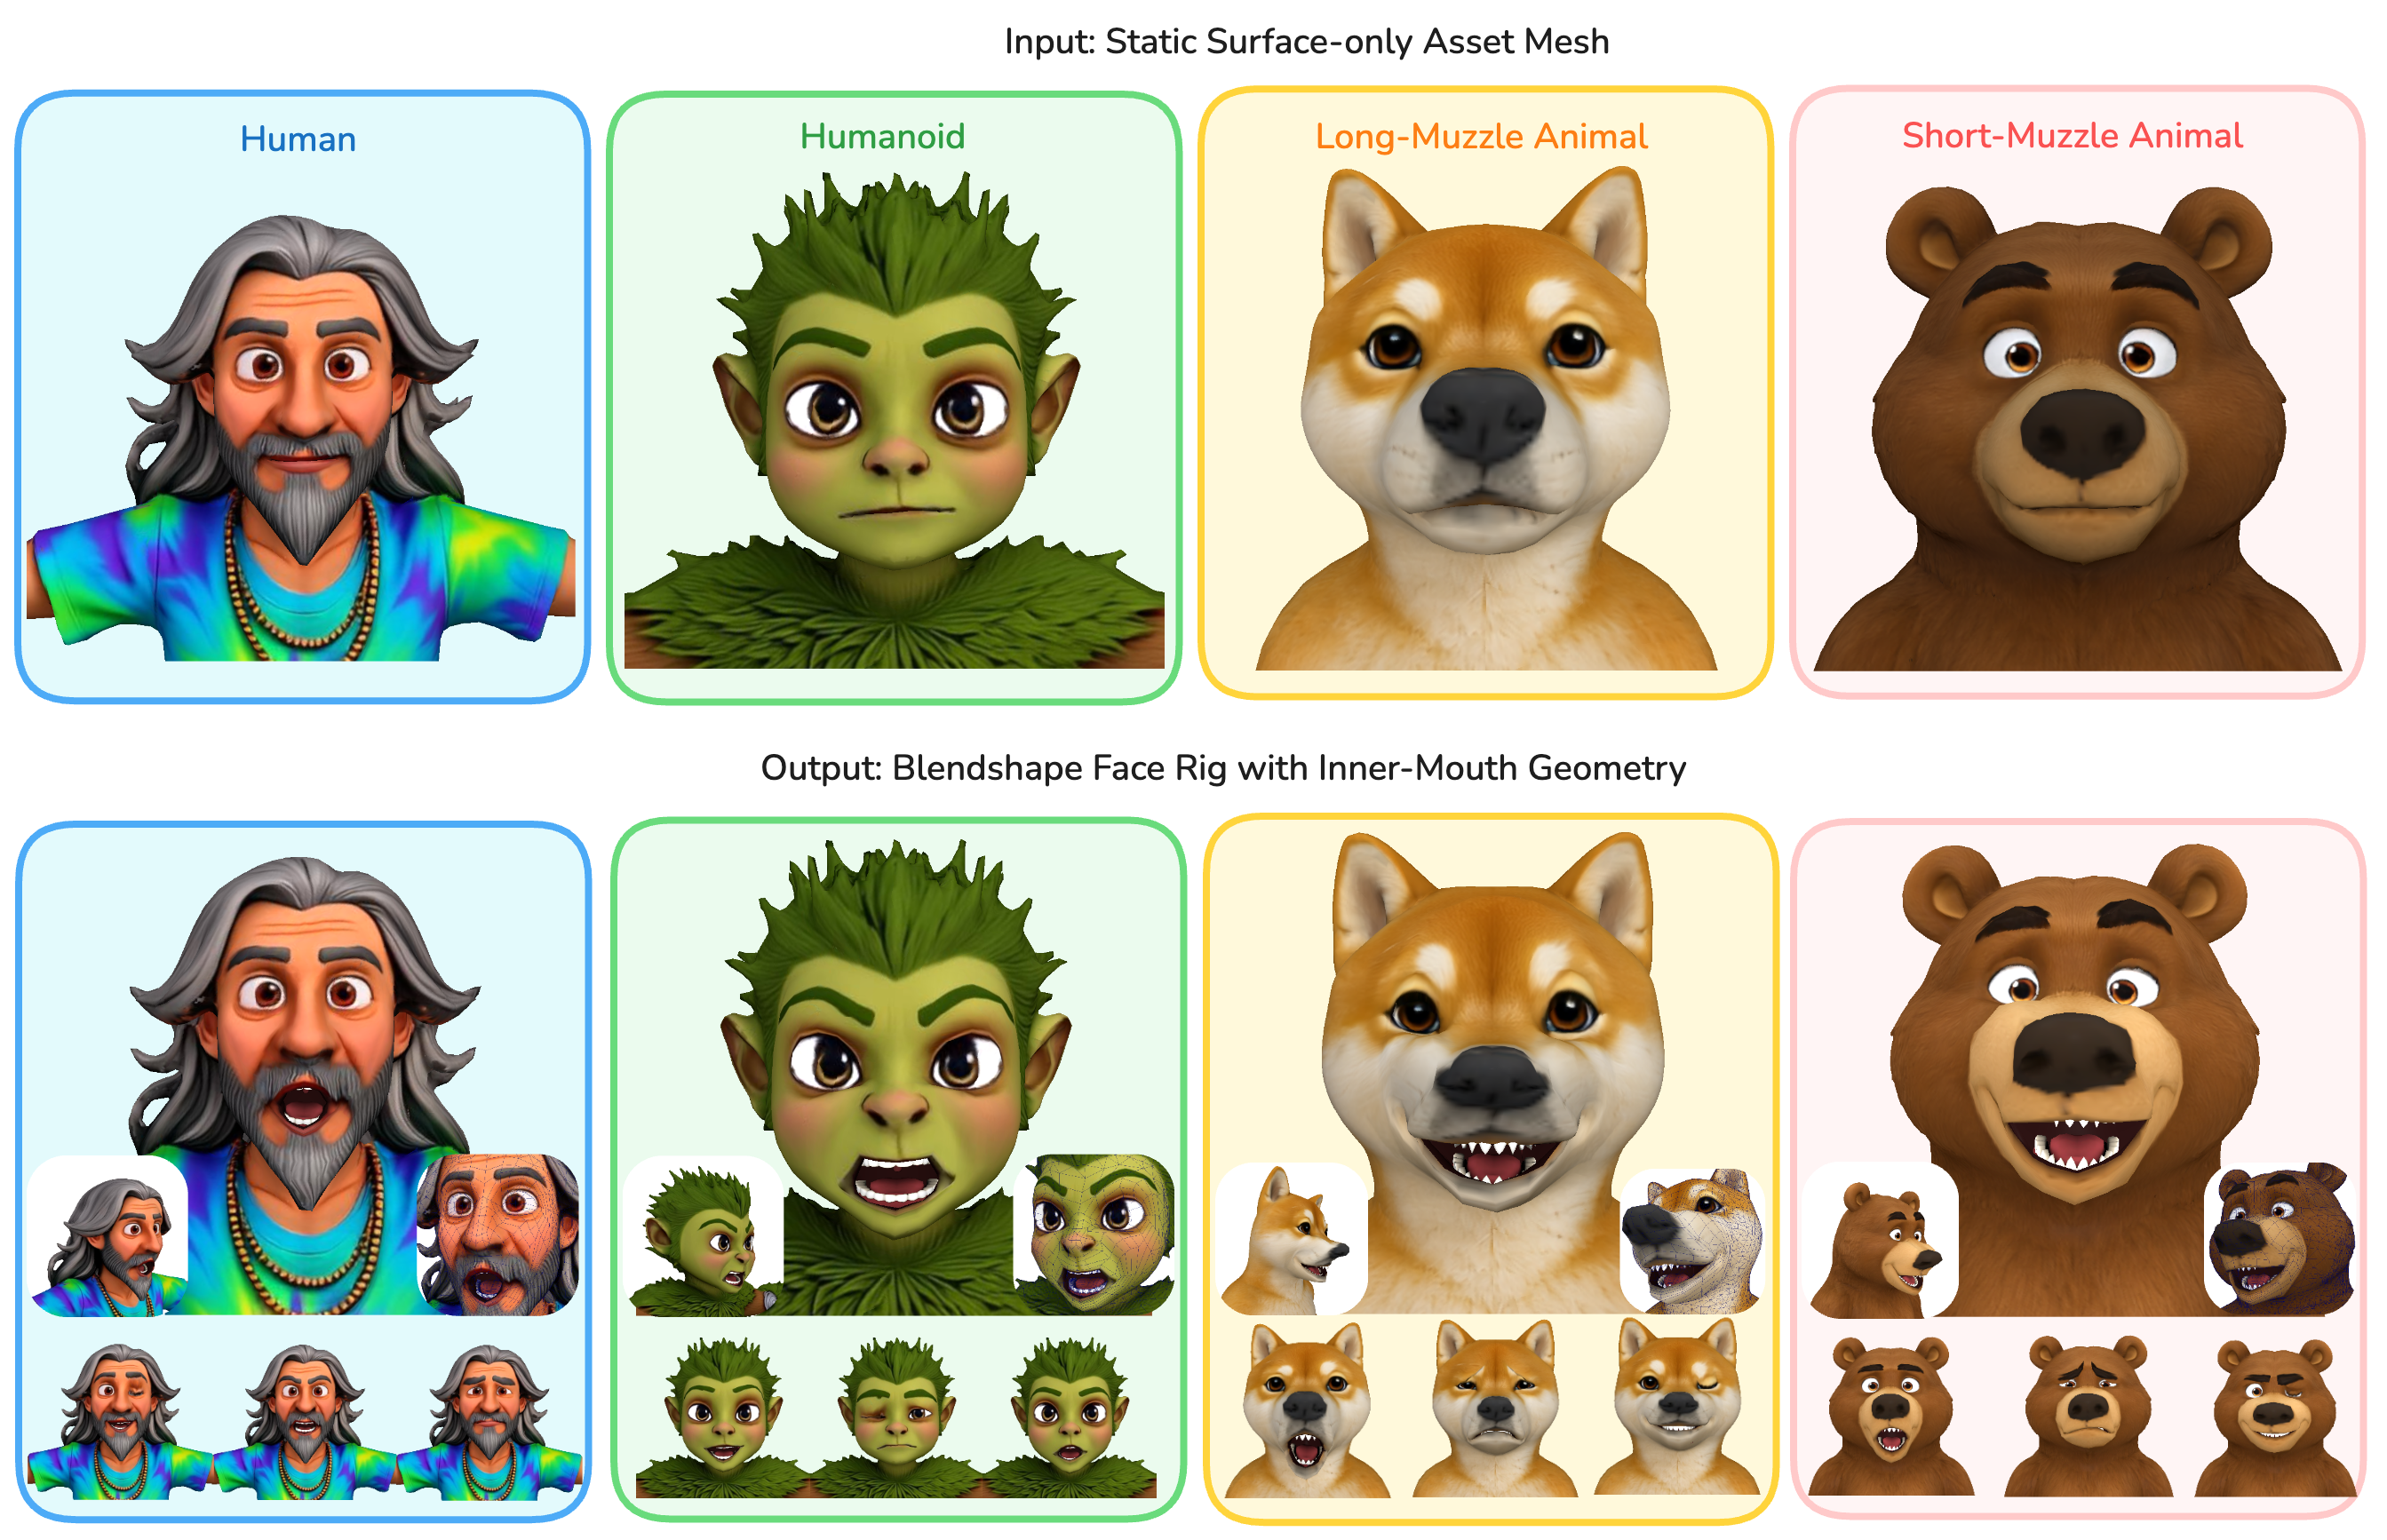
\includegraphics[width=0.95\textwidth]{figures/cover_image.png}
  \caption{OmniFaceRig takes static surface-only 3D meshes with no pre-modeled oral cavity (top row) and fully automatically produces production-ready facial rigs with FACS blendshapes and generated inner-mouth geometry including teeth, gums, and tongue (bottom rows showing expressions and mouth details). The teaser highlights our support for diverse 3D character topologies---humans, humanoids, long-muzzled animals (e.g., dogs), and short-muzzled animals (e.g., bears)---within one unified rigging pipeline. We release Omni-Bench, a benchmark of rigged biped characters spanning humans and animals.}
  \Description{Large teaser showing diverse input static meshes in the top row, with corresponding rigged outputs showing various facial expressions in the rows below.}
  \label{fig:teaser}
\end{teaserfigure}

\maketitle

%% ============================================================
\section{Introduction}
\label{sec:intro}

Facial rigging---creating FACS-based blendshapes and inner-mouth geometry (teeth, gums, and tongue) for 3D character animation---remains one of the most labor-intensive steps in the character production pipeline. A skilled technical artist may spend hours to days sculpting blendshapes for a single character, involving careful topology design, facial landmark placement, expression sculpting, and teeth fitting.

At the same time, 3D asset creation itself has become dramatically more accessible. Recent text-to-3D and image-to-3D methods can generate textured objects or characters directly from prompts or reference images~\cite{poole2023dreamfusion, lin2023magic3d, jun2023shape, liu2023zero123, tang2024make, ren2023make}, and similar capabilities are increasingly available in commercial 3D-generation tools. However, these systems primarily produce static surface meshes and textures. For characters, the generated assets are often plausible as visual meshes but are not animation-ready facial rigs: they typically lack FACS controls, robust facial topology for deformation, and the oral-cavity geometry required for inner-mouth-aware expressions. This makes generated characters natural inputs to an automatic rigging pipeline, but not substitutes for such a pipeline.

Existing rigging solutions address parts of this problem but remain incomplete and, in practice, only \emph{semi-automatic}. Deformation transfer~\cite{sumner2004deformation} and parametric face models~\cite{cao2014facewarehouse, li2017learning} enable facial rig creation but assume compatible mesh topologies, require manual landmark annotation, and are designed exclusively for human faces. Inner-mouth geometry (teeth, gums, and tongue) is particularly costly to author because the input mesh normally contains no corresponding interior surfaces: in production pipelines, teeth, gums, and tongue are almost universally placed and tuned by hand, and manually tuned or human-specific teeth templates routinely fail on stylized or non-human faces. To our knowledge, \emph{no existing system delivers a fully automatic, end-to-end pipeline that produces FACS blendshapes with newly generated inner-mouth geometry from a static surface-only mesh}---let alone across both human and non-human topologies.

We present \textbf{OmniFaceRig}, an end-to-end pipeline for face auto-rigging \textbf{across diverse 3D character topologies}---including humans, humanoids, long-muzzled animals (e.g., dogs, wolves, foxes), and short-muzzled animals (e.g., cats, bears, rabbits, tigers). These animal labels describe coarse facial topology for template selection rather than biological taxonomy: long-muzzled characters have elongated, forward-protruding snouts, while short-muzzled characters have compact or nearly absent snouts. Given a static surface-only 3D mesh with no pre-modeled oral cavity, OmniFaceRig produces a production-ready facial rig with up to 155 FACS blendshapes, procedurally generated inner-mouth geometry (teeth, gums, and tongue), and re-packed UV/texture---all \textbf{fully automatic with no manual intervention at any stage}. In particular, OmniFaceRig eliminates the manual inner-mouth placement, landmark annotation, user-provided templates, and per-asset template setup that bottleneck prior pipelines, allowing the entire facial rig to be generated directly from the input mesh. Our key contributions are:

\begin{enumerate}
  \item To our knowledge, the first \textbf{fully automatic, end-to-end face auto-rigging pipeline} that starts from a static surface-only input mesh and requires no manual inner-mouth placement, landmark annotation, user-provided templates, or per-asset template setup.
  \item \textbf{Inner-mouth-aware rig construction}: OmniFaceRig procedurally generates teeth, gums, tongue, and oral-cavity support geometry that are absent from the input mesh, then integrates them with FACS blendshape transfer using ARAP+SDF fitting and collision-aware deformation.
  \item \textbf{Omni-Bench}: to our knowledge, the first open-source benchmark of 1,000 biped 3D characters with FACS facial blendshapes and inner-mouth geometry (teeth, gums, and tongue), spanning humans (realistic + humanoid, 13 occupations), cats (10 breeds), and dogs (10 breeds) with up to 12 appearance variations---all in T-pose and all rigged by OmniFaceRig.
  \item Generalization across \textbf{diverse non-human topologies}: our method rigs long-muzzled animals (dogs, wolves, foxes, etc.) and short-muzzled animals (cats, bears, rabbits, tigers, etc.) via a small library of topology-specific templates with a nose-landmark-free design and ARAP+SDF teeth placement, demonstrating that the same pipeline transfers from humans to animals without architectural changes.
\end{enumerate}

%% ============================================================
\section{Related Work}
\label{sec:related}

% Method comparison table at top of Related Work section
\begin{table*}[t]
\centering
\caption{Comparison of facial auto-rigging methods. OmniFaceRig is the only compared method achieving fully automatic blendshape generation with no per-asset setup, supporting disconnected components including inner-mouth geometry (teeth, gums, and tongue), and generalizing across diverse human and animal character topologies. ``No Per-Asset Setup'' means no user-provided template, manual landmarking, or per-character fitting adjustment at inference time.}
\label{tab:method_comparison}
\resizebox{\textwidth}{!}{
\begin{tabular}{lccccccc}
\toprule
\textbf{Method} & \textbf{Cross-Topology} & \textbf{No Manual Landmarks} & \textbf{No Per-Asset Setup} & \textbf{Output Format} & \textbf{Disconnected Parts} & \textbf{Inner Mouth} & \textbf{Animal Support} \\
\midrule
Deformation Transfer~\cite{sumner2004deformation} & \xmark & \xmark & \xmark & Mesh & \xmark & \xmark & \xmark \\
Example-Based~\cite{li2010example} & \xmark & \xmark & \xmark & Blendshapes & \xmark & \xmark & \xmark \\
Li et al.~\cite{li2020dynamic} & \xmark & \xmark & \xmark & Blendshapes & \xmark & \xmark & \xmark \\
Chandran et al.~\cite{chandran2022shape} & \cmark & \xmark & \xmark & Mesh & \xmark & \xmark & \xmark \\
NFR~\cite{qin2023neural} & \cmark & \cmark & \cmark & Mesh / Latent & \xmark & \xmark & \xmark \\
NFDT~\cite{chandran2025neural} & \cmark & \cmark & \cmark & Blendshapes & \xmark & \xmark & Limited \\
NFS~\cite{cha2025neural} & \cmark & \cmark & \cmark & Skinning Weights & \cmark & \xmark & \xmark \\
RigAnyFace~\cite{ma2025riganyface} & \cmark & \cmark & \cmark & Blendshapes & \cmark & \xmark & \xmark \\
\midrule
\textbf{OmniFaceRig (Ours)} & \cmark & \cmark & \cmark & \textbf{Blendshapes} & \cmark & \cmark & \cmark \\
\bottomrule
\end{tabular}
}
\end{table*}

\begin{figure*}[t]
  \centering
  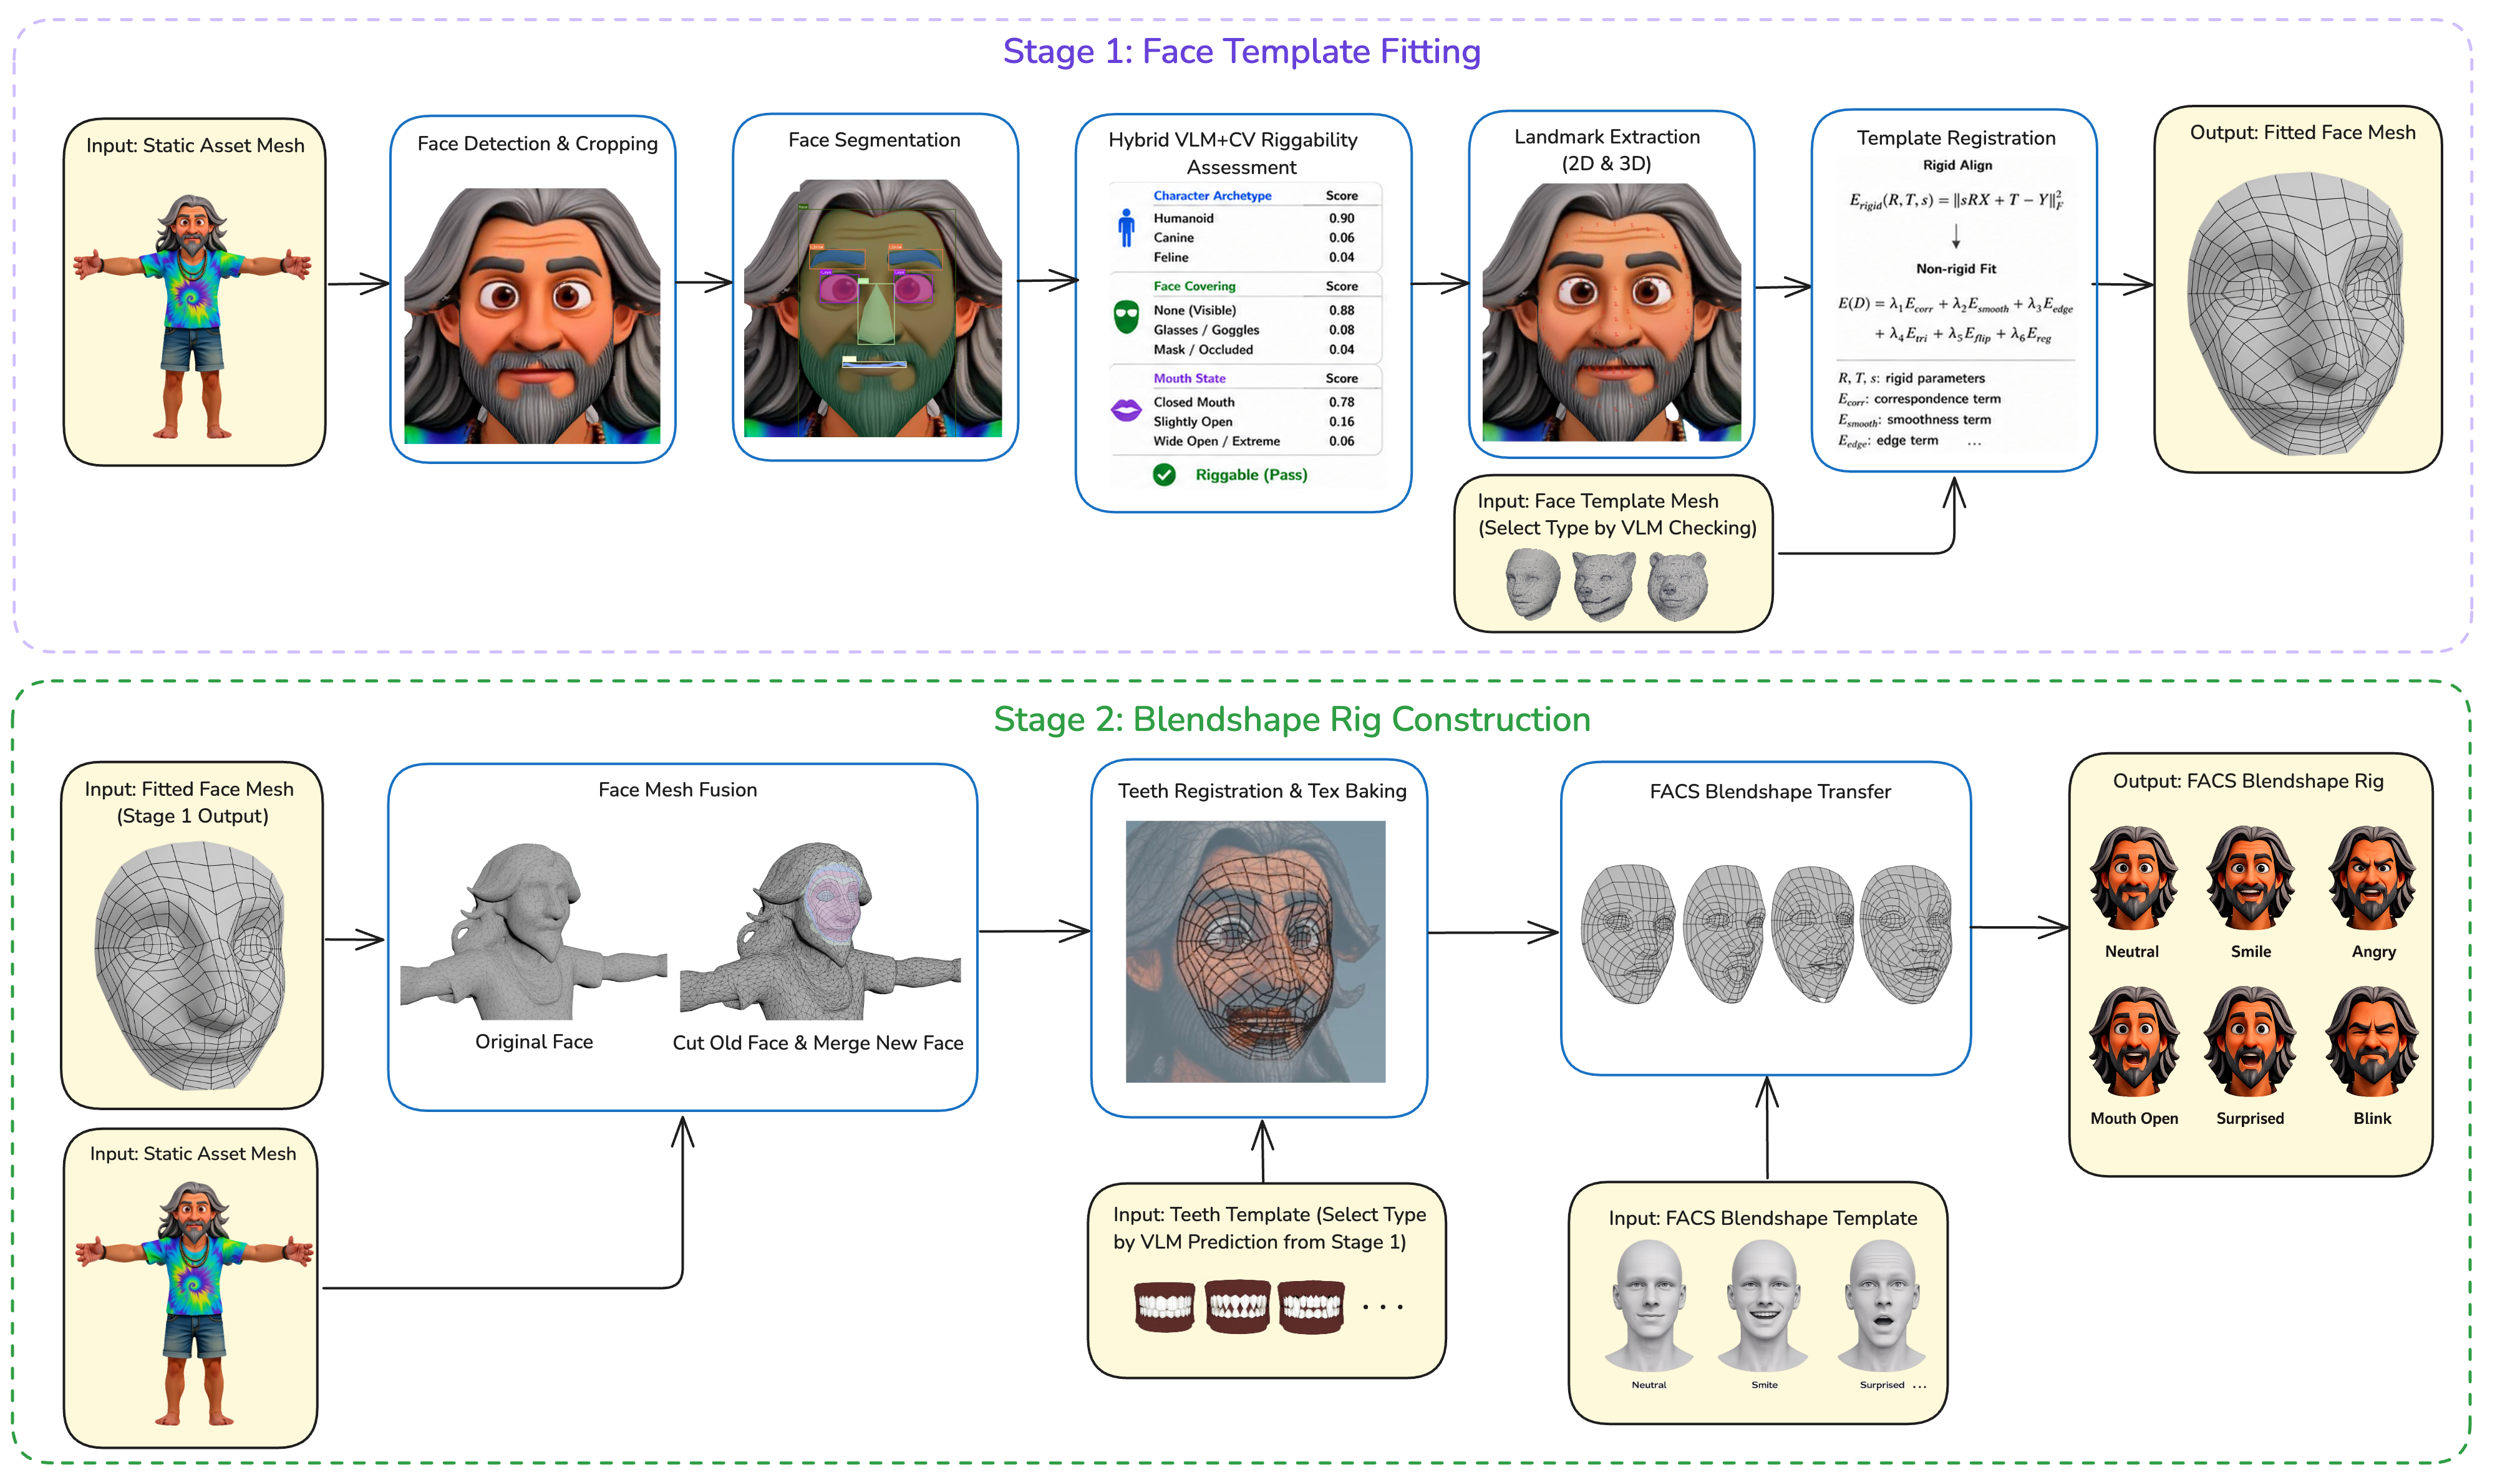
\includegraphics[width=\textwidth]{figures/pipeline.png}
  \caption{OmniFaceRig pipeline architecture. The pipeline consists of two stages. \textbf{Stage~1: Face Template Fitting} takes a static surface-only 3D mesh, performs face detection/cropping, face segmentation, VLM+CV riggability assessment, landmark extraction, and dense keypoint-driven rigid + non-rigid template registration, producing a fitted template mesh aligned to the input face. \textbf{Stage~2: Blendshape Rig Construction} takes the fitted template and constructs a production-ready FACS blendshape rig through face mesh fusion, generated teeth registration and texture baking, and FACS blendshape transfer, producing inner-mouth geometry (teeth, gums, and tongue) and re-packed UV/texture that are not present in the input.}
  \Description{Pipeline diagram showing the two-stage face auto-rigging workflow: Stage 1 (Face Template Fitting) followed by Stage 2 (Blendshape Rig Construction).}
  \label{fig:pipeline}
\end{figure*}

\subsection{3D Asset and Character Generation}

Text-to-3D and image-to-3D generation have rapidly lowered the barrier to creating 3D assets. Methods such as DreamFusion~\cite{poole2023dreamfusion}, Magic3D~\cite{lin2023magic3d}, Shap-E~\cite{jun2023shape}, and Zero-1-to-3~\cite{liu2023zero123} generate textured objects from language or image inputs, while character-focused systems such as Make-it-vivid~\cite{tang2024make} and Make-a-character~\cite{ren2023make} target animatable or stylized 3D characters. Similar capabilities are also increasingly available in commercial 3D-generation services, making static character asset creation accessible to non-expert users. However, these systems primarily target visible geometry and appearance. Their outputs are generally static surface assets, often without production facial topology, FACS controls, or interior oral-cavity geometry. Our work is complementary: OmniFaceRig takes such generated surface meshes as input and converts them into animation-ready, inner-mouth-aware facial rigs.

\subsection{Parametric Face Models vs.\ Blendshape Rigging}

Parametric face models provide statistical representations of human facial geometry. The 3D Morphable Model (3DMM)~\cite{blanz1999morphable}, FaceWarehouse~\cite{cao2014facewarehouse}, and FLAME~\cite{li2017learning} established linear shape spaces for face reconstruction. Extensions include multilinear models~\cite{brunton2014multilinear, vlasic2006face} that factor identity and expression, and disentangled representations~\cite{abrevaya2019decoupled, jiang2019disentangled} that separate shape components for more flexible control. Methods like CoMA~\cite{ranjan2018generating} and DECA~\cite{feng2021learning} leverage these models to reconstruct animatable faces from images. However, parametric models are bound to a fixed topology and blendshape set, and cannot be applied to novel characters with arbitrary topologies, stylized proportions, or non-human features.

In contrast, production pipelines rely on FACS~\cite{ekman1978facial} and blendshape rigging~\cite{lewis2014practice, lewis2010direct}, which offer animators intuitive, localized control while preserving character-specific geometry~\cite{seol2011artist, kavan2024compressed}. Orvalho et al.~\cite{orvalho2012facial} provide a comprehensive survey of facial rigging techniques, covering the evolution from manual sculpting to semi-automatic methods. On the representation side, spectral methods have also been explored for compact animation representations~\cite{wang2015spectral}. Our method follows this production paradigm, generating FACS blendshapes for arbitrary target meshes.

\subsection{Traditional and Learning-Based Facial Auto-Rigging}

\textbf{Traditional methods.} Noh and Neumann~\cite{noh2001expression} introduced expression cloning via vertex displacement transfer. Sumner and Popovi\'{c}~\cite{sumner2004deformation} proposed deformation transfer using triangle affine transformations---the foundational technique our system builds upon. Orvalho et al.~\cite{orvalho2008transferring} extended this to transfer rigs across different face models. Li et al.~\cite{li2010example} further developed example-based facial rigging. Seol et al.~\cite{seol2012spacetime} introduced spacetime expression cloning for blendshapes. Liu et al.~\cite{liu2011framework} proposed a framework for locally retargeting and rendering facial performance. Ribera et al.~\cite{ribera2017facial} addressed retargeting with automatic range of motion alignment. These methods achieve high quality but require manual correspondence establishment, which does not scale.

\textbf{Learning-based methods.} Li et al.~\cite{li2020dynamic} used CNNs to predict blendshape offsets via geometry images. Chandran et al.~\cite{chandran2022shape, chandran2020semantic} introduced semantic deformation transfer and later utilized transformers for topology-independent shape transfer~\cite{chandran2022local}. Blendshape editing has also been explored through sketching interfaces~\cite{cetinaslan2020sketching, cetinaslan2020stabilized}. Wang et al.~\cite{wang2023fully} proposed BSGen for automatic blendshape generation, and Ming et al.~\cite{ming2024high} introduced high-quality mesh blendshape generation from face videos via neural inverse rendering. On the representation side, MeshCNN~\cite{hanocka2019meshcnn} and DiffusionNet~\cite{sharp2022diffusionnet} provide mesh-native learned features that benefit downstream tasks. Neural Face Rigging (NFR)~\cite{qin2023neural} pioneered neural deformation for in-the-wild facial meshes but is limited to human faces and cannot handle disconnected components. FaBRig~\cite{zhu2024fabrig} proposes a cloth-simulated transferable 3D face parameterization. Neural Facial Deformation Transfer (NFDT)~\cite{chandran2025neural} uses a decoder-only transformer for high-fidelity transfer. Neural Face Skinning (NFS)~\cite{cha2025neural} proposes mesh-agnostic skinning. RigAnyFace~\cite{ma2025riganyface} represents the current state-of-the-art, using 2D supervision to scale training with unlabeled data. Most recently, CANRig~\cite{canrig2026} introduces cross-attention mechanisms for neural face rigging with variable local control, and ControlFace~\cite{jang2025controlface} harnesses 3DMM-conditioned rendering for flexible face rigging. Zero-shot approaches~\cite{wang2023zeroshot} and portrait animation methods~\cite{yang2024megactor} have also been explored for stylized characters. DreamFace~\cite{zhang2023dreamface} generates animatable 3D faces under text guidance. As summarized in Table~\ref{tab:method_comparison}, our method addresses critical gaps: inner-mouth modeling (teeth, gums, and tongue) and non-humanoid character rigging.

\subsection{Rigging for Non-Humanoid Characters}

Extending facial rigging to animals remains a formidable challenge due to vastly different anatomy~\cite{danieau2019automatic}. On the 3D shape modeling side, SMAL~\cite{zuffi2017menagerie} and BARC~\cite{rueegg2023barc} model quadruped animal shape and pose using category-specific priors. However, these parametric animal models do not address facial rig construction or blendshape generation. For facial landmark detection on non-photorealistic characters, Cheng et al.~\cite{cheng2024stylizedfacepoint} proposed methods for stylized character facial landmark detection, addressing the domain gap between real human faces and artistic character designs. Recent learning-based rigging methods~\cite{qin2023neural, ma2025riganyface} are trained on human datasets with human-centric priors and do not generalize to animal faces. Critically, nearly all existing methods focus on the outer facial surface, ignoring the oral cavity (teeth, gums, tongue). Our approach introduces a robust multi-model segmentation ensemble that identifies facial regions across species, decoupling geometric processing from human-specific priors. OmniFaceRig generates FACS blendshapes that explicitly include inner-mouth geometry (teeth, gums, and tongue) for both humans and animals.

%% ============================================================
\section{Omni-Bench: Benchmark Dataset}
\label{sec:benchmark}

To facilitate future research in automatic facial rigging, we release \textbf{Omni-Bench}, to our knowledge the first open-source benchmark of biped 3D characters with FACS facial blendshapes and inner-mouth geometry (teeth, gums, and tongue). All released assets are selected from inputs that pass the initial VLM+CV riggability screen, are processed by OmniFaceRig, and are provided in biped T-pose with generated rig outputs.

\begin{table*}[t]
\centering
\caption{Comparison of 3D facial and character datasets. To our knowledge, Omni-Bench is the first dataset providing FACS blendshapes with inner-mouth geometry (teeth, gums, and tongue) for both human and animal full-character assets, along with text-to-3D generation pipeline data.}
\label{tab:dataset_comparison}
\resizebox{\textwidth}{!}{
\begin{tabular}{lccccccc}
\toprule
\textbf{Dataset} & \textbf{Year} & \textbf{Total Models} & \textbf{Species} & \textbf{FACS Blendshapes} & \textbf{Inner Mouth} & \textbf{Full Character} & \textbf{Text + 2D Image} \\
\midrule
BFM~\cite{paysan20093d} & 2009 & 200 & Human & \xmark & \xmark & \xmark & \xmark \\
CoMA~\cite{ranjan2018generating} & 2018 & 144 & Human & \xmark & \xmark & \xmark & \xmark \\
VOCASET~\cite{cudeiro2019capture} & 2019 & 12 (4D) & Human & \xmark & \xmark & \xmark & \xmark \\
FaceScape~\cite{zhu2023facescape} & 2020 & 16,940 & Human & \xmark & \xmark & \xmark & \xmark \\
ICT FaceKit~\cite{li2020learning} & 2020 & 1 (Parametric) & Human & \cmark & \cmark & \xmark & \xmark \\
Multiface~\cite{wuu2022multiface} & 2022 & 13 (Multi-view) & Human & \xmark & \xmark & \xmark & \xmark \\
RaBit~\cite{luo2023rabit} & 2023 & 1,500 & Human \& Cartoon & \xmark & \xmark & \cmark & \xmark \\
Anymate~\cite{anymate2025} & 2025 & 230,000 & Human \& Animal & \xmark & \xmark & \cmark & \xmark \\
\midrule
\textbf{Omni-Bench (Ours)} & 2026 & \textbf{1,000} & \textbf{Human \& Animal} & \cmark & \cmark & \cmark & \cmark \\
\bottomrule
\end{tabular}
}
\end{table*}

The development of robust facial rigging algorithms relies heavily on high-quality 3D datasets. Early datasets like BFM~\cite{paysan20093d} provided PCA-based morphable models but lacked diverse expressions. FaceScape~\cite{zhu2023facescape, yang2020facescape} significantly advanced the field with 16,940 topologically uniform models, though it only captures the outer facial surface. Multiface~\cite{wuu2022multiface} and VOCASET~\cite{cudeiro2019capture} provide high-quality scans for neural rendering and speech-driven animation, but do not provide FACS blendshape rigs. ICT FaceKit~\cite{li2020learning} offers a detailed morphable model including teeth, gums, and eyes, but as a single parametric model rather than a diverse dataset. Existing large-scale character datasets such as RaBit~\cite{luo2023rabit} and Anymate~\cite{anymate2025} provide many full-character assets, but they do not include FACS facial blendshapes or inner-mouth structures.

Omni-Bench addresses these gaps with \textbf{1,000 rigged biped 3D characters}, split into 500 human and humanoid characters and 500 animals. The human set covers realistic humans across 13 common occupations (astronaut, doctor, firefighter, soldier, chef, pilot, nurse, teacher, police officer, engineer, athlete, musician, scientist) as well as stylized humanoid characters (fantasy, sci-fi, and cyberpunk styles). The animal set is dominated by 150 cats (10 breeds: Persian, Siamese, Maine Coon, Sphynx, Ragdoll, British Shorthair, Bengal, Abyssinian, Scottish Fold, Russian Blue) and 150 dogs (10 breeds: Husky, Pug, Labrador, German Shepherd, Corgi, Poodle, Golden Retriever, Bulldog, Beagle, Dalmatian), plus 200 other common animals amenable to rigging (e.g., bears, mice, tigers, lions, foxes, wolves, rabbits, deer); all of them are provided in biped form like the rest of Omni-Bench. Categories include up to 12 appearance variations. Figure~\ref{fig:omnibench_overview} provides a visual overview of the dataset diversity and topology coverage.

The riggability screen should be interpreted as an input eligibility filter rather than a guarantee of final rigging success. It removes obvious invalid assets---for example, missing faces, severe eye or mouth occlusions, non-standard viewpoints, or unsupported facial topologies---before full processing. A screened asset can still fail during later stages because of segmentation errors, unstable template fitting, or implausible mouth localization. We therefore report final \emph{Success Rate} separately in the experiments as the percentage of screened Omni-Bench inputs for which the full OmniFaceRig pipeline completes and passes final geometric quality checks.

As shown in Table~\ref{tab:dataset_comparison}, Omni-Bench stands out in three critical ways. First, it uniquely supports both human and animal characters within a unified rigging framework. Second, every model is equipped with a complete set of auto-generated FACS blendshapes (up to 155 shapes) that explicitly include teeth, gums, and tongue---a feature absent in nearly all existing large-scale datasets. Third, each asset includes the complete generation pipeline data: the initial text description, intermediate 2D reference image, and final 3D mesh, making it an invaluable resource for text-to-3D generation~\cite{tang2024make, ren2023make} and multimodal research. All assets are in biped T-pose and rigged by OmniFaceRig, providing a consistent and reproducible evaluation baseline.


%% ============================================================
\section{Method}
\label{sec:method}

\subsection{Pipeline Overview}
\label{sec:overview}

OmniFaceRig takes a static surface-only 3D mesh with no pre-modeled oral cavity and produces a production-ready facial rig with FACS blendshapes and inner-mouth geometry (teeth, gums, and tongue) (Figure~\ref{fig:pipeline}). The pipeline is organized into two stages. \textbf{Stage~1: Face Template Fitting} (\S\ref{sec:riggability}--\S\ref{sec:fitting}) lifts the input mesh into a canonical template space through a sequence of steps: we first render the input 3D mesh to a frontal-view character image, then perform face detection and cropping to localize the face region; the cropped face is parsed by a multi-model segmentation ensemble; a hybrid VLM+CV riggability assessment uses visual-semantic predictions together with CV segmentation signals to decide whether to proceed and to select the face/teeth template configuration; 2D and 3D keypoints are extracted from the final segmentation masks; and finally a rigid + non-rigid template registration aligns a canonical face template to the input face, producing a fitted face mesh. \textbf{Stage~2: Blendshape Rig Construction} (\S\ref{sec:blendshape}) takes the fitted template and constructs a production-ready FACS blendshape rig---fusing the fitted face with the original asset, procedurally generating and placing inner-mouth geometry (teeth, gums, and tongue), baking texture into a re-packed UV layout, and transferring blendshape deformations from a canonical rigged template to the asset.


\subsection{Riggability Assessment}
\label{sec:riggability}

Before processing an asset through the rigging pipeline, OmniFaceRig performs an automatic eligibility check. This is critical in production settings where input assets are generated automatically (e.g., from text-to-3D models) and may include characters with no visible face, heavily occluded facial features, non-standard orientations, or facial topologies outside the current template library.

Our riggability assessment is a \textbf{VLM+CV hybrid} system combining two complementary approaches:

\textbf{VLM Understanding.} We render the input 3D mesh from a frontal viewpoint and query a state-of-the-art Vision-Language Model (VLM) to identify: (1) the \emph{character archetype} (human, humanoid, feline, canine, or other); (2) \emph{face covering status} (glasses, goggles, masks, eye patches); and (3) \emph{teeth state} (open mouth, closed mouth, emotional expression). The VLM's flexibility allows easy adaptation to new assessment criteria without retraining. The VLM has two roles. First, it filters out assets that are unlikely to be riggable by the current system, including no-face assets, faces with severe eye or mouth occlusion, and unsupported facial topologies such as highly exaggerated beaked birds or other shapes outside our human, long-muzzle, and short-muzzle template families. Second, for assets that pass this eligibility check, it selects downstream configuration choices: (i) the \emph{face template variant}---one of \emph{human}, \emph{long-muzzle}, or \emph{short-muzzle}---based on the character's facial topology (see \S\ref{sec:fitting}); and (ii) the \emph{teeth archetype} (human, canine, or monster), which Stage~2 (\S\ref{sec:blendshape}) uses for inner-mouth fitting.

\textbf{CV Segmentation Filtering.} After face localization, we compute face segmentation masks using the multi-model ensemble described in \S\ref{sec:segmentation}. Assets where no valid face region is detected, or where the face area falls below a minimum threshold, are filtered out. This CV-based check catches cases where the VLM may be overconfident---for example, detecting a ``face'' on a purely mechanical character with no actual facial geometry.

\textbf{Hybrid Decision.} The final eligibility decision combines VLM predictions with CV filtering results. We evaluate the hybrid approach on a mixed riggability validation set of approximately 500 assets, including Omni-Bench candidates, a subset of a separate benchmark collection, and additional generated or collected examples. This validation set intentionally includes both riggable and non-riggable inputs; metrics compare the automatic checker decision against human ground-truth riggability labels:

\begin{table}[t]
  \caption{Riggability assessment accuracy on a mixed validation set of approximately 500 assets with human ground-truth riggability labels. The hybrid VLM+CV approach achieves the best performance.}
  \label{tab:riggability}
  \begin{tabular}{lccc}
    \toprule
    Method & Accuracy & Recall & F1 \\
    \midrule
    VLM only & 94.69\% & 94.76\% & 94.71\% \\
    CV segmentation filtering only & 76.72\% & 94.87\% & 80.87\% \\
    \textbf{VLM + CV (Ours)} & \textbf{$>$95\%} & \textbf{$>$95\%} & \textbf{$>$95\%} \\
    \bottomrule
  \end{tabular}
\end{table}

The hybrid approach leverages the VLM's strong image understanding for high-level decisions while using CV signals for geometric validation, consistently outperforming either component alone. Additional details on the per-question signal assignment, segmentation-mask checks, and mouth-signal fusion are provided in the supplemental material.

\subsection{Sapiens-Based Segmentation Models}
\label{sec:seg_models}

\subsubsection{Pretraining}

Our learned parser is built on Sapiens-1B~\cite{khirodkar2025sapiens}, a high-resolution ViT encoder pretrained on a large human-centric web corpus. The pretraining objective follows masked reconstruction: only a subset of patches is visible to the encoder, and the model learns to infer the missing image content from context. For dense human understanding, this inductive bias is particularly useful because the representation remains tied to the observed pixels instead of collapsing purely to global invariances. In practice, it preserves the local appearance and boundary cues that matter for rigging---hairlines, eyelids, lip contours, teeth, and inner-mouth structure---while still learning broad human semantics across pose, clothing, illumination, and style variation. We therefore use the pretrained Sapiens encoder as the common initialization for all Sapiens-based segmentation models in OmniFaceRig. We make two adaptations for our setting: first, we pretrain at 512$\times$512 resolution for efficiency and then briefly switch to 1024$\times$1024 resolution to improve high-resolution facial boundary cues; second, we perform mid-stage unsupervised adaptation on 20M curated in-domain stylized character images. The pretraining corpus contains approximately 4B curated realistic human images. In downstream parsing experiments, these adaptations improve segmentation accuracy by 2--3\%, and the in-domain adaptation makes supervised parser training more annotation-efficient.

\subsubsection{Segmentation Fine-Tuning}

Starting from this pretrained encoder, we attach a lightweight three-stage deconvolutional decoder that upsamples the token grid back to dense logits, and fine-tune only this head while keeping the ViT backbone frozen. We deploy two compatible checkpoints that share the same Sapiens-1B encoder but use different label spaces: a 41-class stylized parser for human-like characters and a 38-class humanoid parser for cartoon animals and strongly non-human characters. The stylized vocabulary retains fine face-specific classes such as facial skin, eyebrows, eyes, ears, lips, teeth, tongue, hair, glasses, and occluders, whereas the humanoid vocabulary trades some granularity for improved stability on cats, dogs, and heavily stylized characters.

To make these parsers practical inside the rigging loop, we package them in a lightweight train--export--infer stack with JSON label configurations and TorchScript checkpoints. This lets the same encoder--decoder family serve dataset curation, ablation, and deployment on standard GPU servers without additional infrastructure. At inference time, OmniFaceRig consumes only the face-relevant channels and collapses them into the geometric cues required downstream: face boundary, eyes, nose or muzzle extent, mouth opening, teeth or inner-mouth support, and accessory-aware occlusion regions.



\subsection{Face Detection and Segmentation}
\label{sec:segmentation}

Robust face detection and segmentation are critical prerequisites for template fitting. \textbf{Render and Face Detection.} For each input asset, we first render the 3D mesh from a frontal viewpoint into a 2D character image, then localize and crop the face region; the cropped face image is the input to all subsequent face-parsing modules. \textbf{Multi-Model Segmentation.} While real-time face parsing methods such as BiSeNet~\cite{yu2018bisenet} have achieved strong results on photographic human faces, AI-generated characters exhibit highly stylized proportions and diverse topologies that challenge any single detector or parser. To maximize coverage, we combine the Sapiens-based parsers from \S\ref{sec:seg_models} with two complementary off-the-shelf models and adaptively select the best result for each facial region:

\begin{enumerate}
  \item \textbf{Face Landmark Detection}: A face detection and landmark model providing 68-keypoint facial landmarks with high precision on human and near-human faces. Used as the primary landmark source for eyes, mouth, and face boundary on human characters.
  \item \textbf{Sapiens}~\cite{khirodkar2025sapiens}: The base human parser described in \S\ref{sec:seg_models}. It provides strong human nose, lip, and facial-skin estimates, but degrades on strongly non-human faces because of its human-centric training distribution.
  \item \textbf{SAM 3} (Segment Anything Model 3)~\cite{carion2025sam3}: Building on the Segment Anything foundation~\cite{kirillov2023segment} and its video extension SAM~2~\cite{ravi2024sam2}, SAM~3 is a class-agnostic segmentation foundation model that provides zero-shot segmentation masks from point or box prompts. SAM 3 generalizes well to stylized and non-human faces but produces coarser boundaries compared to landmark-based methods. We use SAM 3 for face region segmentation on characters where face landmark detection and Sapiens fail.
  \item \textbf{Fine-Tuned Sapiens}: Our stylized and humanoid Sapiens checkpoints from \S\ref{sec:seg_models}. The riggability stage selects the 41-class stylized variant for human-like characters and the 38-class humanoid variant for cats, dogs, and heavily stylized assets; these models serve as the primary dense parsers whenever face landmark detection or the base Sapiens model becomes unreliable.
\end{enumerate}

For each input 3D asset, we render the mesh from a frontal viewpoint and run all four models in parallel. The system then \emph{adaptively selects the best detection and segmentation result for each facial part} from the available models. Specifically:
\begin{itemize}
  \item For \emph{human} assets with standard facial proportions, we rely on face landmark detection (higher precision for eyes and mouth) combined with Sapiens face parsing (for nose and skin regions).
  \item For \emph{stylized humanoid} assets where face landmark detection may fail due to exaggerated proportions, the system falls back to the 41-class fine-tuned Sapiens parser, which handles non-standard facial proportions more robustly.
  \item For \emph{animal} assets (felines, canines) where both face landmark detection and standard Sapiens fail, the system uses the 38-class humanoid Sapiens parser (primary) with SAM 3 (fallback) for face boundary and region segmentation.
  \item Automatic fallback is applied at the per-region level: if the preferred model fails for a specific facial part (e.g., nose segmentation on a cat), the system seamlessly switches to the next-best model for that region only.
\end{itemize}

The combined multi-model ensemble achieves a face detection recall of \textbf{nearly 100\%} across our test sets, compared to \textbf{88\%} for the best single model in isolation. This improvement is especially pronounced on challenging cases: animal characters with fur-covered face boundaries, humanoid characters with exaggerated feature proportions, and characters wearing partial face accessories.

\begin{figure}[!htb]
  \centering
  \begin{subfigure}[t]{\linewidth}
    \centering
    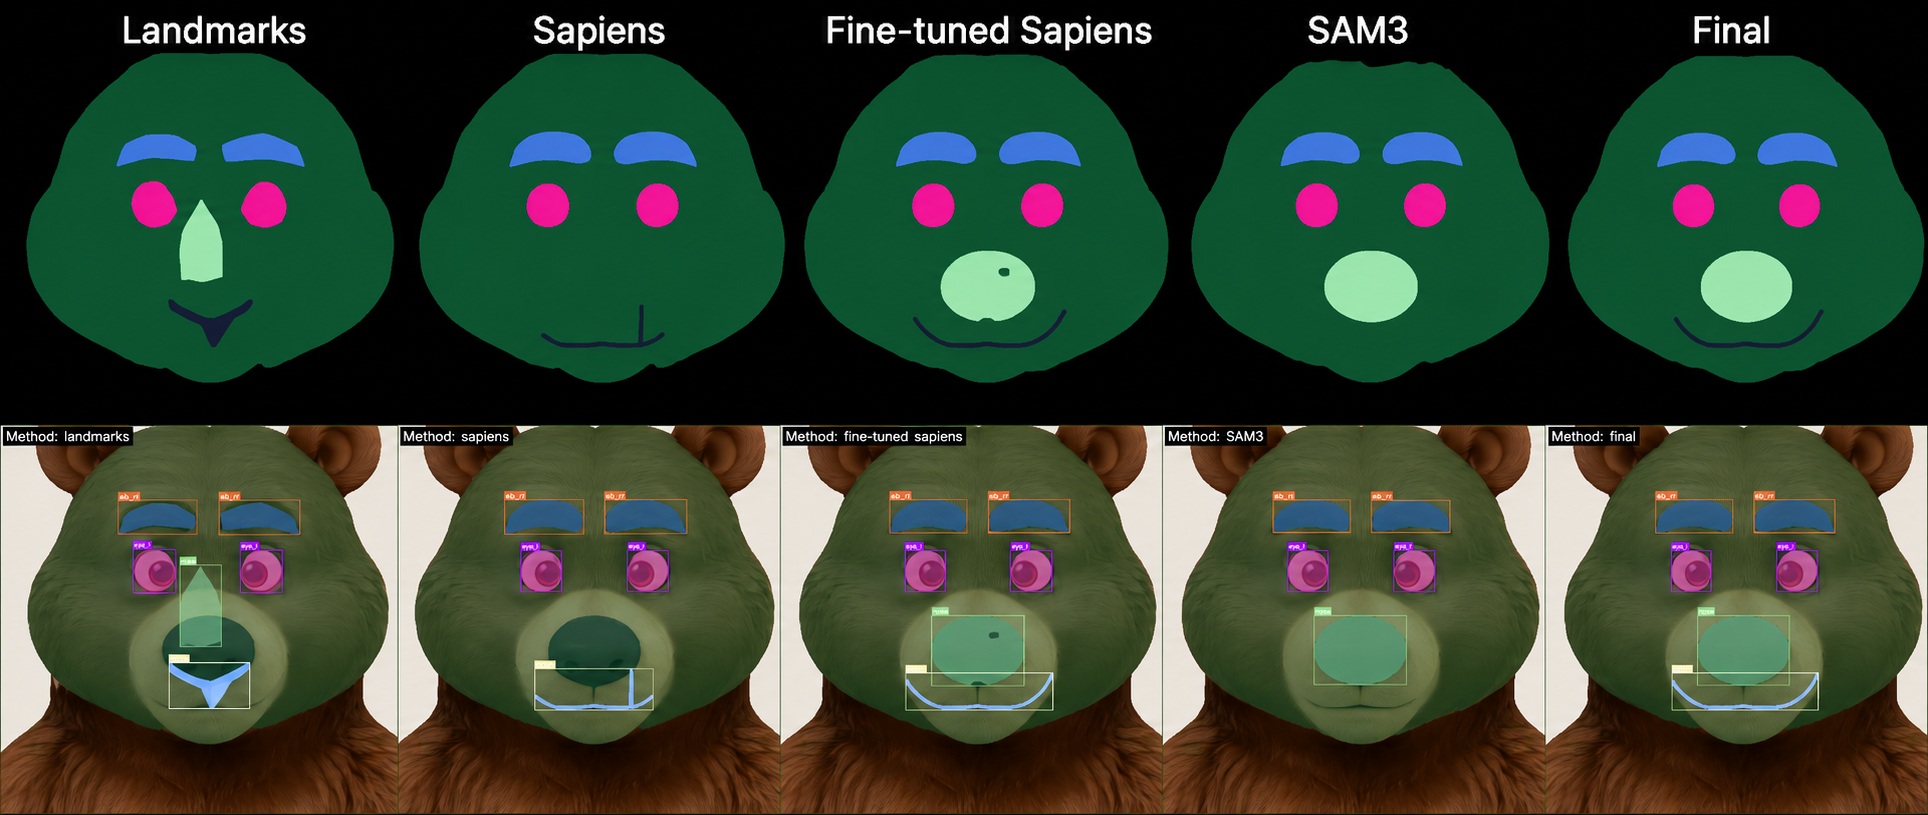
\includegraphics[width=\linewidth]{figures/seg_methods_comp.png}
    \caption{Single-model-dominant case.}
    \label{fig:segmentation_a}
  \end{subfigure}\\[0.4em]
  \begin{subfigure}[t]{\linewidth}
    \centering
    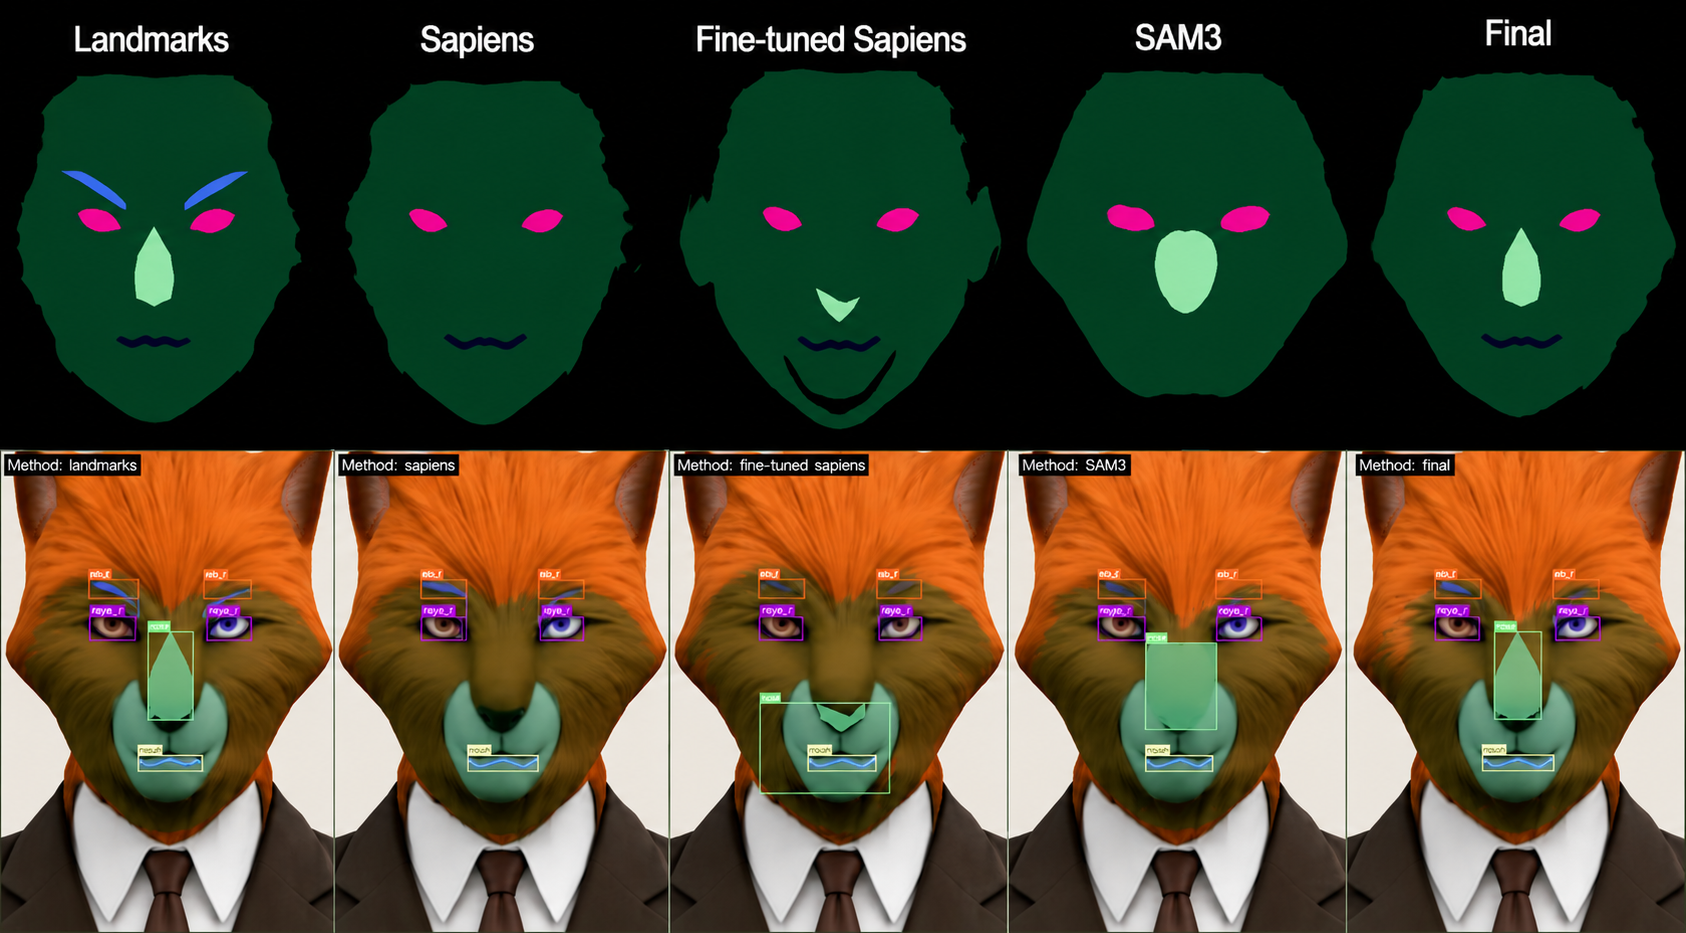
\includegraphics[width=\linewidth]{figures/seg_methods_comp_02.png}
    \caption{Ensemble case (per-region fusion needed).}
    \label{fig:segmentation_b}
  \end{subfigure}
  \caption{Multi-model face detection and segmentation ensemble. Four models run in parallel; the system adaptively selects the best result per facial region. \textbf{(a)} On a bear, fine-tuned Sapiens already produces a reliable parse and the final result mostly inherits from it. \textbf{(b)} On a fox, fine-tuned Sapiens fails (e.g., spuriously detecting two mouths) and no other single model is fully reliable either; the final mask is assembled by picking the best per-region output across the four models.}
  \Description{Two-panel comparison of the multi-model segmentation ensemble: (a) a case where one fine-tuned model dominates, and (b) a case where the final mask is assembled per-region from several models.}
  \label{fig:segmentation}
\end{figure}

\textbf{Landmark Extraction (2D \& 3D).} After segmentation, we extract 2D and 3D keypoints from the final segmentation masks. 2D landmarks for the face boundary, eyes, nose or muzzle, and mouth are read from mask contours and face landmark predictions. We then back-project each 2D landmark onto the input 3D mesh by ray-casting from the rendered camera through the pixel and intersecting the asset surface, yielding the paired 3D position. The resulting 2D + 3D keypoint correspondences are the input to template registration (\S\ref{sec:fitting}).


\subsection{Template Registration}
\label{sec:fitting}

\subsubsection{Template Design}

The core of OmniFaceRig's face fitting stage is a small library of quad-mesh templates with anchor keypoints, designed for robust fitting across diverse character topologies. The anchor keypoints correspond to facial landmarks (eyes, mouth, face boundary) whose 3D positions are computed from the segmentation ensemble output (\S\ref{sec:segmentation}). To accommodate the wide variation in facial shape across topologies, we provide \textbf{three face template variants}, and the VLM (\S\ref{sec:riggability}) automatically selects the appropriate one for each input asset:

\begin{itemize}
  \item \textbf{Human template} --- targets human and humanoid characters with conventional facial proportions (flat-fronted face, defined chin, eyes and mouth on roughly the same plane).
  \item \textbf{Long-muzzle template} --- targets long-muzzled animals with elongated, forward-protruding snouts, such as dogs, wolves, foxes, and horses.
  \item \textbf{Short-muzzle template} --- targets short-muzzled animals with compact or nearly absent snouts, such as cats, bears, rabbits, and tigers.
\end{itemize}

All three templates share three common design principles that make fitting robust across diverse character types:

\begin{itemize}
  \item \textbf{Nose-landmark-free design.} Anchor target positions are computed by uniformly sampling along the corresponding segmentation-mask boundary, and nose anchors are particularly fragile under this scheme for two compounding reasons. First, nose segmentation accuracy itself is consistently low on animal faces (feline noses are small and short; canine noses merge into the muzzle) and on many stylized humanoids, so the underlying mask is unreliable. Second, even when the nose mask is plausible, the nose contour tends to be small, irregular, or weakly defined, so uniform boundary sampling yields unstable keypoints that do not correspond across assets. We therefore exclude the nose region from the anchor keypoints entirely; the nose vertices are positioned by the optimization itself, guided by the surrounding border, eye, and mouth anchors. This makes fitting independent of nose segmentation quality, and the resulting nose region naturally adapts to actual face proportions---compact for cats, elongated for dogs, standard for humans.
  \item \textbf{Decoupled fitting and animated topology.} The fitting template (optimized for keypoint correspondence) and the animated topology (designed with radial edge loops around eyes and mouth for muscle-direction deformation) are maintained as separate meshes linked by UV correspondence. This decoupling allows independent optimization: the fitting template can be modified for better landmark matching without affecting the animation-quality edge flow, and vice versa.
  \item \textbf{Minimum region fitting.} The template adheres to the convex hull of facial features rather than extending to the neck and chin. This ``minimum region'' design produces tighter fits, reduces artifacts at the face-asset merge boundary, and improves robustness on characters with unusual neck or chin geometry (e.g., characters with armor, scarves, or elongated chins).
\end{itemize}

\subsubsection{Keypoint Computation and Fallback Mechanisms}

The template fitting relies on \textbf{dense facial keypoint correspondences} between the 68 template anchor vertices and their target positions on the input asset face. These target positions are computed from the segmentation ensemble: eye corners and contours from face landmark detection or fine-tuned Sapiens, mouth corners from landmark detection, and face boundary from segmentation mask edges.

To achieve \textbf{zero invalid keypoint errors} across all test assets, we implement three fallback mechanisms:
\begin{enumerate}
  \item \textbf{Mesh-surface fallback for border keypoints.} After correcting invalid border keypoints to the nearest face mask boundary, some corrected positions still fail 3D projection because the face mask and the actual mesh surface do not perfectly overlap. When a border keypoint has no valid 3D position after mask-boundary correction, we search for the nearest pixel on the actual mesh surface and compute the 3D position directly from the mesh geometry at that pixel.
  \item \textbf{3D anchor-based fallback.} When a keypoint's 2D-to-3D projection fails (e.g., the 2D position lands in an area with no mesh geometry), we fall back to computing its 3D position from the already-resolved 3D positions of neighboring anchor keypoints, maintaining a running map of resolved positions so that later keypoints can reference those resolved earlier.
  \item \textbf{Adaptive eye mask selection.} Both segmentation-based and landmark-based eye masks can contribute to the face boundary computation, but including both can produce an overly large convex hull. We use only one eye mask source, selected adaptively: human assets use landmark-based eyes (higher precision), non-human assets use segmentation-based eyes (more robust), with auto-fallback if the preferred source is unavailable.
\end{enumerate}

\subsubsection{Template Fitting Optimization}

Given the template mesh and computed keypoint correspondences, the fitting stage deforms the template to match the input asset via a two-stage optimization.

\emph{Stage 1: Global Rigid Alignment.} We find the best rigid transformation (rotation $\mathbf{R}$, scale $s$, translation $\mathbf{t}$) aligning template keypoints $\mathbf{v}_i$ to asset keypoints $\mathbf{p}_i$ by minimizing:
\begin{equation}
  E_{\text{rigid}} = \sum_{i \in \mathcal{K}} \| s\mathbf{R}\mathbf{v}_i + \mathbf{t} - \mathbf{p}_i \|^2
\end{equation}
where $\mathcal{K}$ is the set of corresponding keypoints.

\emph{Stage 2: Per-Vertex Non-Rigid Deformation.} We optimize per-vertex displacements $\mathbf{d}_i$ for all vertices to minimize a composite energy function:
\begin{equation}
  E(\mathbf{D}) = \lambda_1 E_{\text{corr}} + \lambda_2 E_{\text{smooth}} + \lambda_3 E_{\text{edge}} + \lambda_4 E_{\text{tri}} + \lambda_5 E_{\text{flip}} + \lambda_6 E_{\text{reg}}
\end{equation}
where each energy term controls a different aspect of data fitting or geometric regularization to make this fitting pipeline robust to various input cases. The terms are defined as follows:

\textbf{Correspondence energy} ($E_{\text{corr}}$) is the main data term that pulls the template keypoints toward their corresponding asset keypoints:
\begin{equation}
  E_{\text{corr}} = \sum_{i \in \mathcal{K}} \mathcal{H}(\| \mathbf{v}'_i - \mathbf{p}_i \|)
\end{equation}
where $\mathbf{v}'_i = \mathbf{v}_i + \mathbf{d}_i$ represents the deformed template vertex positions, $\mathbf{p}_i$ represents target landmark points, and $\mathcal{H}$ is a robust penalty function such as a Huber loss to ignore outliers.

\textbf{Smoothness energy} ($E_{\text{smooth}}$) enforces smooth deformations by encouraging neighboring vertices connected by a mesh edge $\mathcal{E}$ to move in a similar way:
\begin{equation}
  E_{\text{smooth}} = \sum_{(i,j) \in \mathcal{E}} \| \mathbf{d}_i - \mathbf{d}_j \|^2
\end{equation}

\textbf{Edge-length preservation energy} ($E_{\text{edge}}$) encourages the deformation to remain locally rigid by preserving original edge lengths up to global scale:
\begin{equation}
  E_{\text{edge}} = \sum_{(i,j) \in \mathcal{E}} \left( \| \mathbf{v}'_i - \mathbf{v}'_j \| - \| \mathbf{v}_i - \mathbf{v}_j \| \right)^2
\end{equation}

\textbf{Triangle shape preservation energy} ($E_{\text{tri}}$) preserves local triangle shapes more strongly than edge-length preservation alone and prevents skinny or sheared triangles:
\begin{equation}
  E_{\text{tri}} = \sum_{t \in \mathcal{T}} \| \mathbf{G}_t - \mathbf{G}'_t \|_F^2
\end{equation}
where $\mathbf{G}_t$ and $\mathbf{G}'_t$ denote triangle shape matrices encoding the edge lengths and angles before and after deformation, respectively.

\textbf{Triangle flip penalty} ($E_{\text{flip}}$) penalizes orientation reversal and reduces triangle flips and foldovers to prevent self-intersections:
\begin{equation}
  E_{\text{flip}} = \sum_{t \in \mathcal{T}} \max(0, -\mathbf{n}_t \cdot \mathbf{n}'_t)^3
\end{equation}
where $\mathbf{n}_t$ and $\mathbf{n}'_t$ denote triangle normals before and after deformation, respectively.

\textbf{Offset regularization energy} ($E_{\text{reg}}$) discourages unnecessarily large deformations and improves numerical stability:
\begin{equation}
  E_{\text{reg}} = \sum_i \| \mathbf{d}_i \|^2
\end{equation}

For normalized meshes, this optimization achieves \textbf{near-zero alignment error} ($<10^{-5}$). The nose-landmark-free template design and triangle flip penalty ensure \textbf{zero crashes} across all animal assets in Omni-Bench, naturally adapting to diverse face proportions (compact for cats, elongated for dogs) without category-specific tuning.


\subsection{Blendshape Rig Construction}
\label{sec:blendshape}

Given the fitted face mesh produced by Stage~1 (\S\ref{sec:fitting}), Stage~2 constructs a production-ready FACS blendshape rig in three steps. The original asset is assumed to provide only the visible surface and source textures, with no pre-existing teeth, gums, tongue, or oral-cavity geometry. Stage~2 therefore consumes three additional inputs: the original static asset mesh (for surrounding geometry and source textures), the teeth template selected by the VLM in Stage~1 (\S\ref{sec:riggability}), and a canonical FACS blendshape template.

\textbf{(1) Face Mesh Fusion.} The fitted template positions are first transferred to a high-quality animated topology mesh via UV correspondence, then reprojected onto the input character geometry. Eye regions are inset using virtual eyeball centers (computed via Procrustes alignment of eyelid vertices) to allow eyelid closure without self-intersection. The prepared template then replaces the face region on the original mesh: a 3D convex hull is computed for a subtractive boolean (cut out the old face), the template border vertices are stitched to the remaining mesh boundary via closest-point welding, and small-edge collapse removes degenerate polygons (merge in the new face). This ensures proper radial topology flow around eyes and mouth for high-quality facial deformation.

\textbf{(2) Teeth Registration and Texture Baking.} \emph{Teeth registration.} Since generated character meshes contain no interior mouth geometry, OmniFaceRig synthesizes the missing inner-mouth structures (teeth, gums, and tongue) from the teeth template selected by the VLM in Stage~1. The selected teeth template is warped to the fitted mouth interior using Radial Basis Function (RBF) deformation, followed by a rigid transform with non-uniform scale. To prevent teeth protrusion---especially critical for muzzled animal faces---we employ \textbf{As-Rigid-As-Possible (ARAP)} deformation~\cite{sorkine2007rigid} for initial placement, then iteratively refine using a \textbf{Signed Distance Field (SDF)}: the convex hull of the teeth geometry is converted to an SDF, and any face mesh points intersecting the teeth volume are smoothly pushed outward along the SDF gradient. Gum and tongue geometry are fitted simultaneously, connected to the inner mouth surface. This two-stage approach (ARAP + SDF) reliably prevents teeth-face intersections both at rest and during expression activation. \emph{Texture baking.} After mesh merging, UV islands are re-packed using an automated UV layout solver to maximize packing area with no overlap between shells, with sufficient padding to prevent visible seams during MipMap rendering. The face region is scaled up to allocate approximately 10$\times$ more texel density than non-face regions, ensuring high-quality facial texture at all LOD levels. The original texture is resampled onto the new UV layout using a vectorized approach: for each pixel in the output texture, we find the barycentric coordinate and primitive ID on the merged mesh's UV layout, convert to world-space position, find the closest point on the original mesh, and sample the source texture at the corresponding UV. Teeth geometry uses a separate texture channel.

\textbf{(3) FACS Blendshape Transfer.} Facial expressions are created by transferring blendshapes from the canonical FACS blendshape template to the merged character mesh using \textbf{sparse deformation transfer}~\cite{sumner2004deformation}. For each reference shape, triangle-level affine deformations are computed and transferred to the target mesh's triangle structure, preserving character-specific geometry while reproducing the expression. The transferred shapes are applied to the merged mesh using Point Deform with Delta Mush smoothing to blend into adjacent non-template regions. Post-processing includes: (a) \emph{contact-aware eyelid closure}~\cite{lewis2014practice}---upper eyelid vertices are snapped to lower lids and edge-relaxed for closed-eye shapes; (b) \emph{eye gaze shapes}---rotation around the virtual eyeball center; (c) \emph{collision-aware deformation transfer}---a collision term prevents lip-teeth intersections during expression shapes. Teeth geometry follows jaw-related shapes via RBF warping converted to rigid transforms. The system supports three configurable shape-set tiers selected per application: \textbf{Core} (13 shapes) for basic dialog and emotion on mobile characters, \textbf{Additional} (46 shapes) for finer muscle control suitable for mid-fidelity game characters, and \textbf{Full} (155 shapes) for production VR applications where expression fidelity is paramount.

The output of Stage~2 is the final \textbf{FACS blendshape rig}, ready to be driven by arbitrary expression weights at run-time. Additional implementation details for face-region fusion, inner-mouth construction, UV/texture transfer, and expression post-processing are provided in the supplemental material.


%% ============================================================
\section{Experiments}
\label{sec:experiments}

\subsection{Setup}

We evaluate OmniFaceRig on the full Omni-Bench dataset (Section~\ref{sec:benchmark}). All inference-time rigging and evaluation experiments use a single NVIDIA A100 GPU; segmentation model fine-tuning is an offline training step and uses the separate multi-GPU setup described below.


\subsection{Implementation Details}
\label{subsec:implementation}

\textbf{Sapiens Pre-Training.} We use Sapiens-1B~\cite{khirodkar2025sapiens} as the base segmentation backbone for all Sapiens-based parsers in OmniFaceRig. Following \S\ref{sec:seg_models}, the encoder is initialized with masked-reconstruction pretraining: we first train at 512$\times$512 resolution for efficiency, then briefly switch to 1024$\times$1024 resolution for high-resolution facial boundary cues. The pretraining corpus contains approximately 4B curated realistic human images. We then perform a mid-stage unsupervised adaptation on 20M in-domain stylized character images. In our downstream parsing experiments, these two stages improve segmentation accuracy by 2--3\%, and the in-domain adaptation makes the subsequent supervised parser training more annotation-efficient.

\textbf{Fine-Tuned Sapiens Training.} To extend Sapiens' face parsing capability to stylized and non-human characters, we construct a custom training dataset of approximately 10,000 annotated 2D images covering humans, humanoids, and animal species such as felines, canines, ursines, and other stylized creatures, all rendered in frontal T-pose. Starting from the pretrained encoder, we attach a lightweight three-stage deconvolutional decoder and train two compatible parser heads: a 41-class stylized parser for human-like characters and a 38-class humanoid parser for cartoon animals and strongly non-human characters. For evaluation and geometric fitting, these fine-grained labels are collapsed into the face-relevant cues consumed by the rigging pipeline: face boundary, eyes, nose or muzzle extent, mouth opening, teeth or inner-mouth support, and accessory-aware occlusion regions.

During fine-tuning, we freeze the Sapiens-1B ViT encoder to preserve its open-world visual features and train only the segmentation decoder heads. Training uses AdamW with a learning rate of $1 \times 10^{-4}$, cosine decay with 500 warmup steps, batch size 16, and class-balanced cross-entropy loss for imbalanced facial regions. Training runs for 50 epochs on 8$\times$ NVIDIA A100 GPUs, taking approximately 24 hours. We apply standard data augmentation: random horizontal flip, color jitter, random rotation ($\pm$15$^\circ$), and random scale (0.8--1.2$\times$).

The fine-tuned parsers achieve a mean Intersection-over-Union (mIoU) of \textbf{87.3\%} on our held-out test set after collapsing predictions to the rigging-relevant facial cues, compared to 62.1\% for the original Sapiens parser. The improvement is most pronounced on animal faces: cat face mIoU improves from 31.2\% to 84.5\%, and dog face mIoU from 28.7\% to 81.9\%, while human face mIoU remains stable (89.1\% $\rightarrow$ 91.2\%).

\subsection{Evaluation Metrics and Baselines}
\label{subsec:metrics}

Drawing upon the evaluation protocols established by recent state-of-the-art methods~\cite{ma2025riganyface, qin2023neural, cha2025neural}, we employ a comprehensive set of metrics. We use \textbf{Mean Absolute Error (MAE)} and \textbf{95th-Percentile Vertex Error (MAE Q95)} to measure the mean and worst-case per-vertex Euclidean distance between the predicted expression mesh and ground truth (normalized to a unit sphere). \textbf{Penetration Rate} measures the percentage of penetrating vertices between inner-mouth components (teeth, gums, and tongue) and the outer facial surface. To quantify pipeline robustness, we introduce \textbf{Success Rate}, tracking the percentage of successfully rigged assets among screened candidate inputs that have passed the VLM+CV riggability checker. Finally, \textbf{Processing Latency} measures the end-to-end execution time in seconds.

For evaluation datasets, we utilize subsets of the ICT FaceKit~\cite{li2020dynamic} and Multiface~\cite{wuu2022multiface} datasets for standard humanoid comparisons. For in-the-wild and non-humanoid evaluation, we utilize our proposed Omni-Bench.

We benchmark our method against the most relevant recent baselines: \textbf{Neural Face Rigging (NFR)}~\cite{qin2023neural} (a pioneering neural method for in-the-wild facial meshes), \textbf{Deformation Transfer (DT)}~\cite{sumner2004deformation} (the classic geometric baseline), and \textbf{RigAnyFace}~\cite{ma2025riganyface} (the current state-of-the-art supporting disconnected components). 

\subsection{Quantitative Results}

\begin{table}[t]
  \caption{Quantitative comparison with state-of-the-art methods on 200 human/humanoid heads. Baseline numbers (DT, NFR, RigAnyFace) are taken from RigAnyFace~\cite{ma2025riganyface}. All meshes are normalized to a unit sphere (radius 1\,m). $^*$Requires manual correspondence annotations.}
  \label{tab:quant_comparison}
  \small
  \begin{tabular}{l@{\hspace{4pt}}c@{\hspace{4pt}}c@{\hspace{4pt}}c}
    \toprule
    Method & MAE$\downarrow$ & Q95$\downarrow$ & Penet.$\downarrow$ \\
    & (mm) & (mm) & (\%) \\
    \midrule
    DT~\cite{sumner2004deformation}$^*$ & 2.93 & 8.41 & -- \\
    NFR~\cite{qin2023neural} & 2.77 & 7.21 & -- \\
    RigAnyFace~\cite{ma2025riganyface} & 1.01 & 2.94 & 0.17 \\
    \textbf{OmniFaceRig (Ours)} & \textbf{0.85} & \textbf{2.50} & \textbf{0.05} \\
    \bottomrule
  \end{tabular}
\end{table}

Table~\ref{tab:quant_comparison} presents the quantitative comparison against state-of-the-art methods on 200 human/humanoid heads. OmniFaceRig achieves the lowest mean vertex error (MAE: 0.85\,mm) and worst-case error (MAE Q95: 2.50\,mm), outperforming RigAnyFace by 16\% and 15\% respectively. Our collision-aware deformation transfer reduces the penetration rate to 0.05\%, a $3.4\times$ improvement over RigAnyFace, ensuring clean separation between inner-mouth components (teeth, gums, and tongue) and the outer facial surface. Beyond alignment quality, OmniFaceRig also runs the full pipeline reliably on this screened evaluation set, with the riggability checker filtering out unsupported inputs and the remaining assets all producing complete rigs. Note that OmniFaceRig performs strictly more work than the compared baselines (face fusion, inner-mouth synthesis, UV/texture re-bake, and FACS transfer in addition to surface alignment), and its 20--30\,s end-to-end runtime on a single A100 GPU includes data I/O, which itself accounts for roughly 10--15\,s of the total; the per-stage breakdown is reported in \S\ref{sec:latency}.

\begin{table}[t]
  \caption{Quantitative comparison on a 300-asset human + humanoid subset of Omni-Bench. We restrict this evaluation to humans and stylized humanoids because DT and NFR are designed for human facial topology and do not generalize to non-human characters. RigAnyFace~\cite{ma2025riganyface} is not included here because its code is not publicly available, so it cannot be re-evaluated on Omni-Bench. $^*$Requires manual correspondence annotations.}
  \label{tab:omnibench_comparison}
  \small
  \begin{tabular}{l@{\hspace{4pt}}c@{\hspace{4pt}}c@{\hspace{4pt}}c@{\hspace{4pt}}c}
    \toprule
    Method & MAE$\downarrow$ & Q95$\downarrow$ & Penet.$\downarrow$ & Succ.$\uparrow$ \\
    & (mm) & (mm) & (\%) & (\%) \\
    \midrule
    DT~\cite{sumner2004deformation}$^*$ & 3.12 & 9.05 & -- & 82.4 \\
    NFR~\cite{qin2023neural} & 2.95 & 8.11 & -- & 85.1 \\
    \textbf{OmniFaceRig (Ours)} & \textbf{0.92} & \textbf{2.71} & \textbf{0.08} & \textbf{99.0} \\
    \bottomrule
  \end{tabular}
\end{table}

Table~\ref{tab:omnibench_comparison} presents the evaluation on a 300-asset subset of Omni-Bench that combines realistic humans and stylized humanoids. We restrict this comparison to humans and humanoids because DT and NFR are designed for human facial topology and do not produce meaningful results on non-human characters; including them on Omni-Bench animal assets would not be a fair comparison. The evaluated inputs have first passed the initial VLM+CV riggability screen, which filters out assets with missing faces, severe occlusions, non-standard orientations, or unsupported facial topologies. On this human + humanoid subset, traditional methods like DT and early learning-based methods like NFR struggle with the stylized humanoid characters, while OmniFaceRig maintains sub-millimeter alignment error, a low penetration rate, and a near-perfect \textbf{99.0\%} final rigging success rate. Across the broader Omni-Bench set including animals, OmniFaceRig further exhibits \textbf{zero crashes} on all animal assets thanks to our multi-stage keypoint fallback mechanisms. Figure~\ref{fig:qualitative_results} shows qualitative rigging results across diverse character types and expression frames; additional qualitative grids covering more identities, styles, and topology families are provided in the supplemental material.

% --- Small inline figures placed first so their [!htb] placement is not blocked
% by the page-only [!p] floats below.
\begin{figure}[!htb]
  \centering
  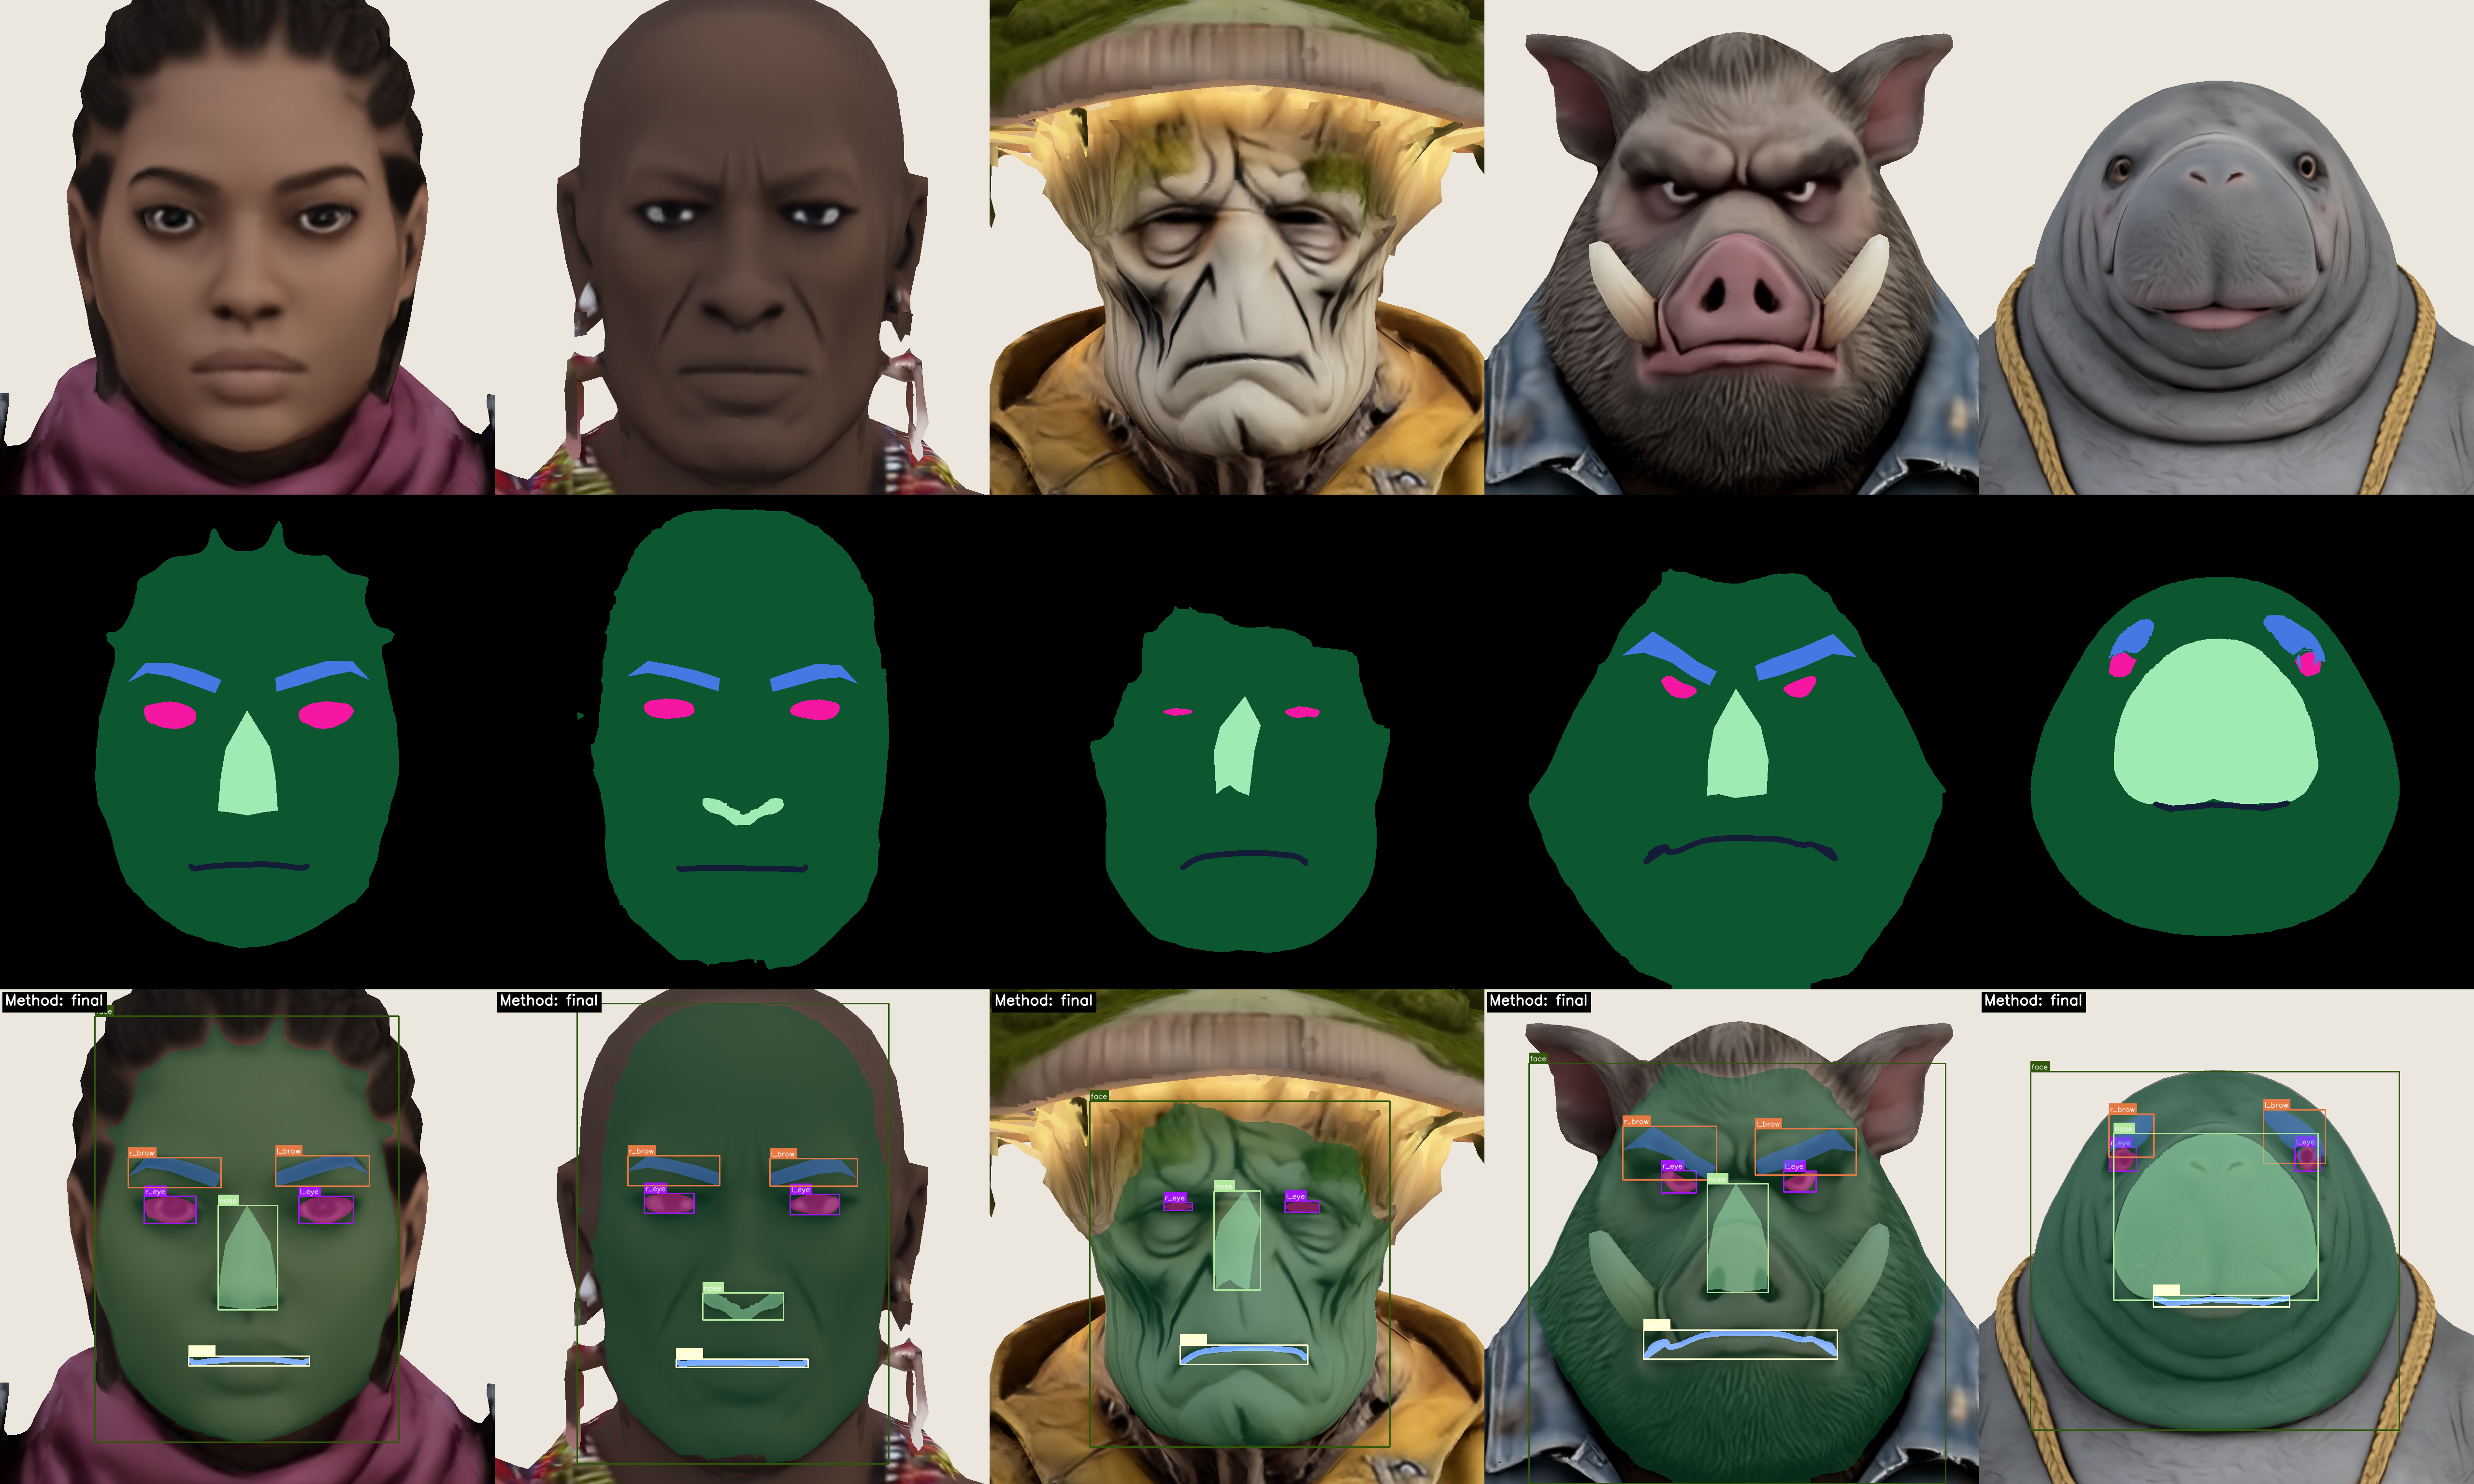
\includegraphics[width=\linewidth]{figures/nose_comp.png}
  \caption{\textbf{Why nose anchors are unreliable.} Across five representative assets the nose region exhibits dramatic variation in both detection quality and contour shape. \textbf{From left to right:} (1) a human with a clean, well-detected nose (a positive baseline); (2) a human where nose detection outright fails; (3) a stylized humanoid where detection returns a mask but the contour is oddly shaped; (4) an animal where detection succeeds but the mask has the wrong overall nose shape; and (5) an animal where detection technically succeeds but the nose mask merges with the mouth into an irregular contour. \textbf{Rows (top to bottom):} input asset render; final nose segmentation mask; asset render with the mask overlaid. Even when detection succeeds, the strongly varying nose contour means that uniformly-sampled boundary keypoints do not correspond across assets, motivating our nose-landmark-free template design (\S\ref{sec:fitting}).}
  \Description{Nose comparison figure showing five characters arranged in columns and three rows (input render, segmentation mask, and overlay).}
  \label{fig:nose_rationale}
\end{figure}

\begin{figure}[!htb]
  \centering
  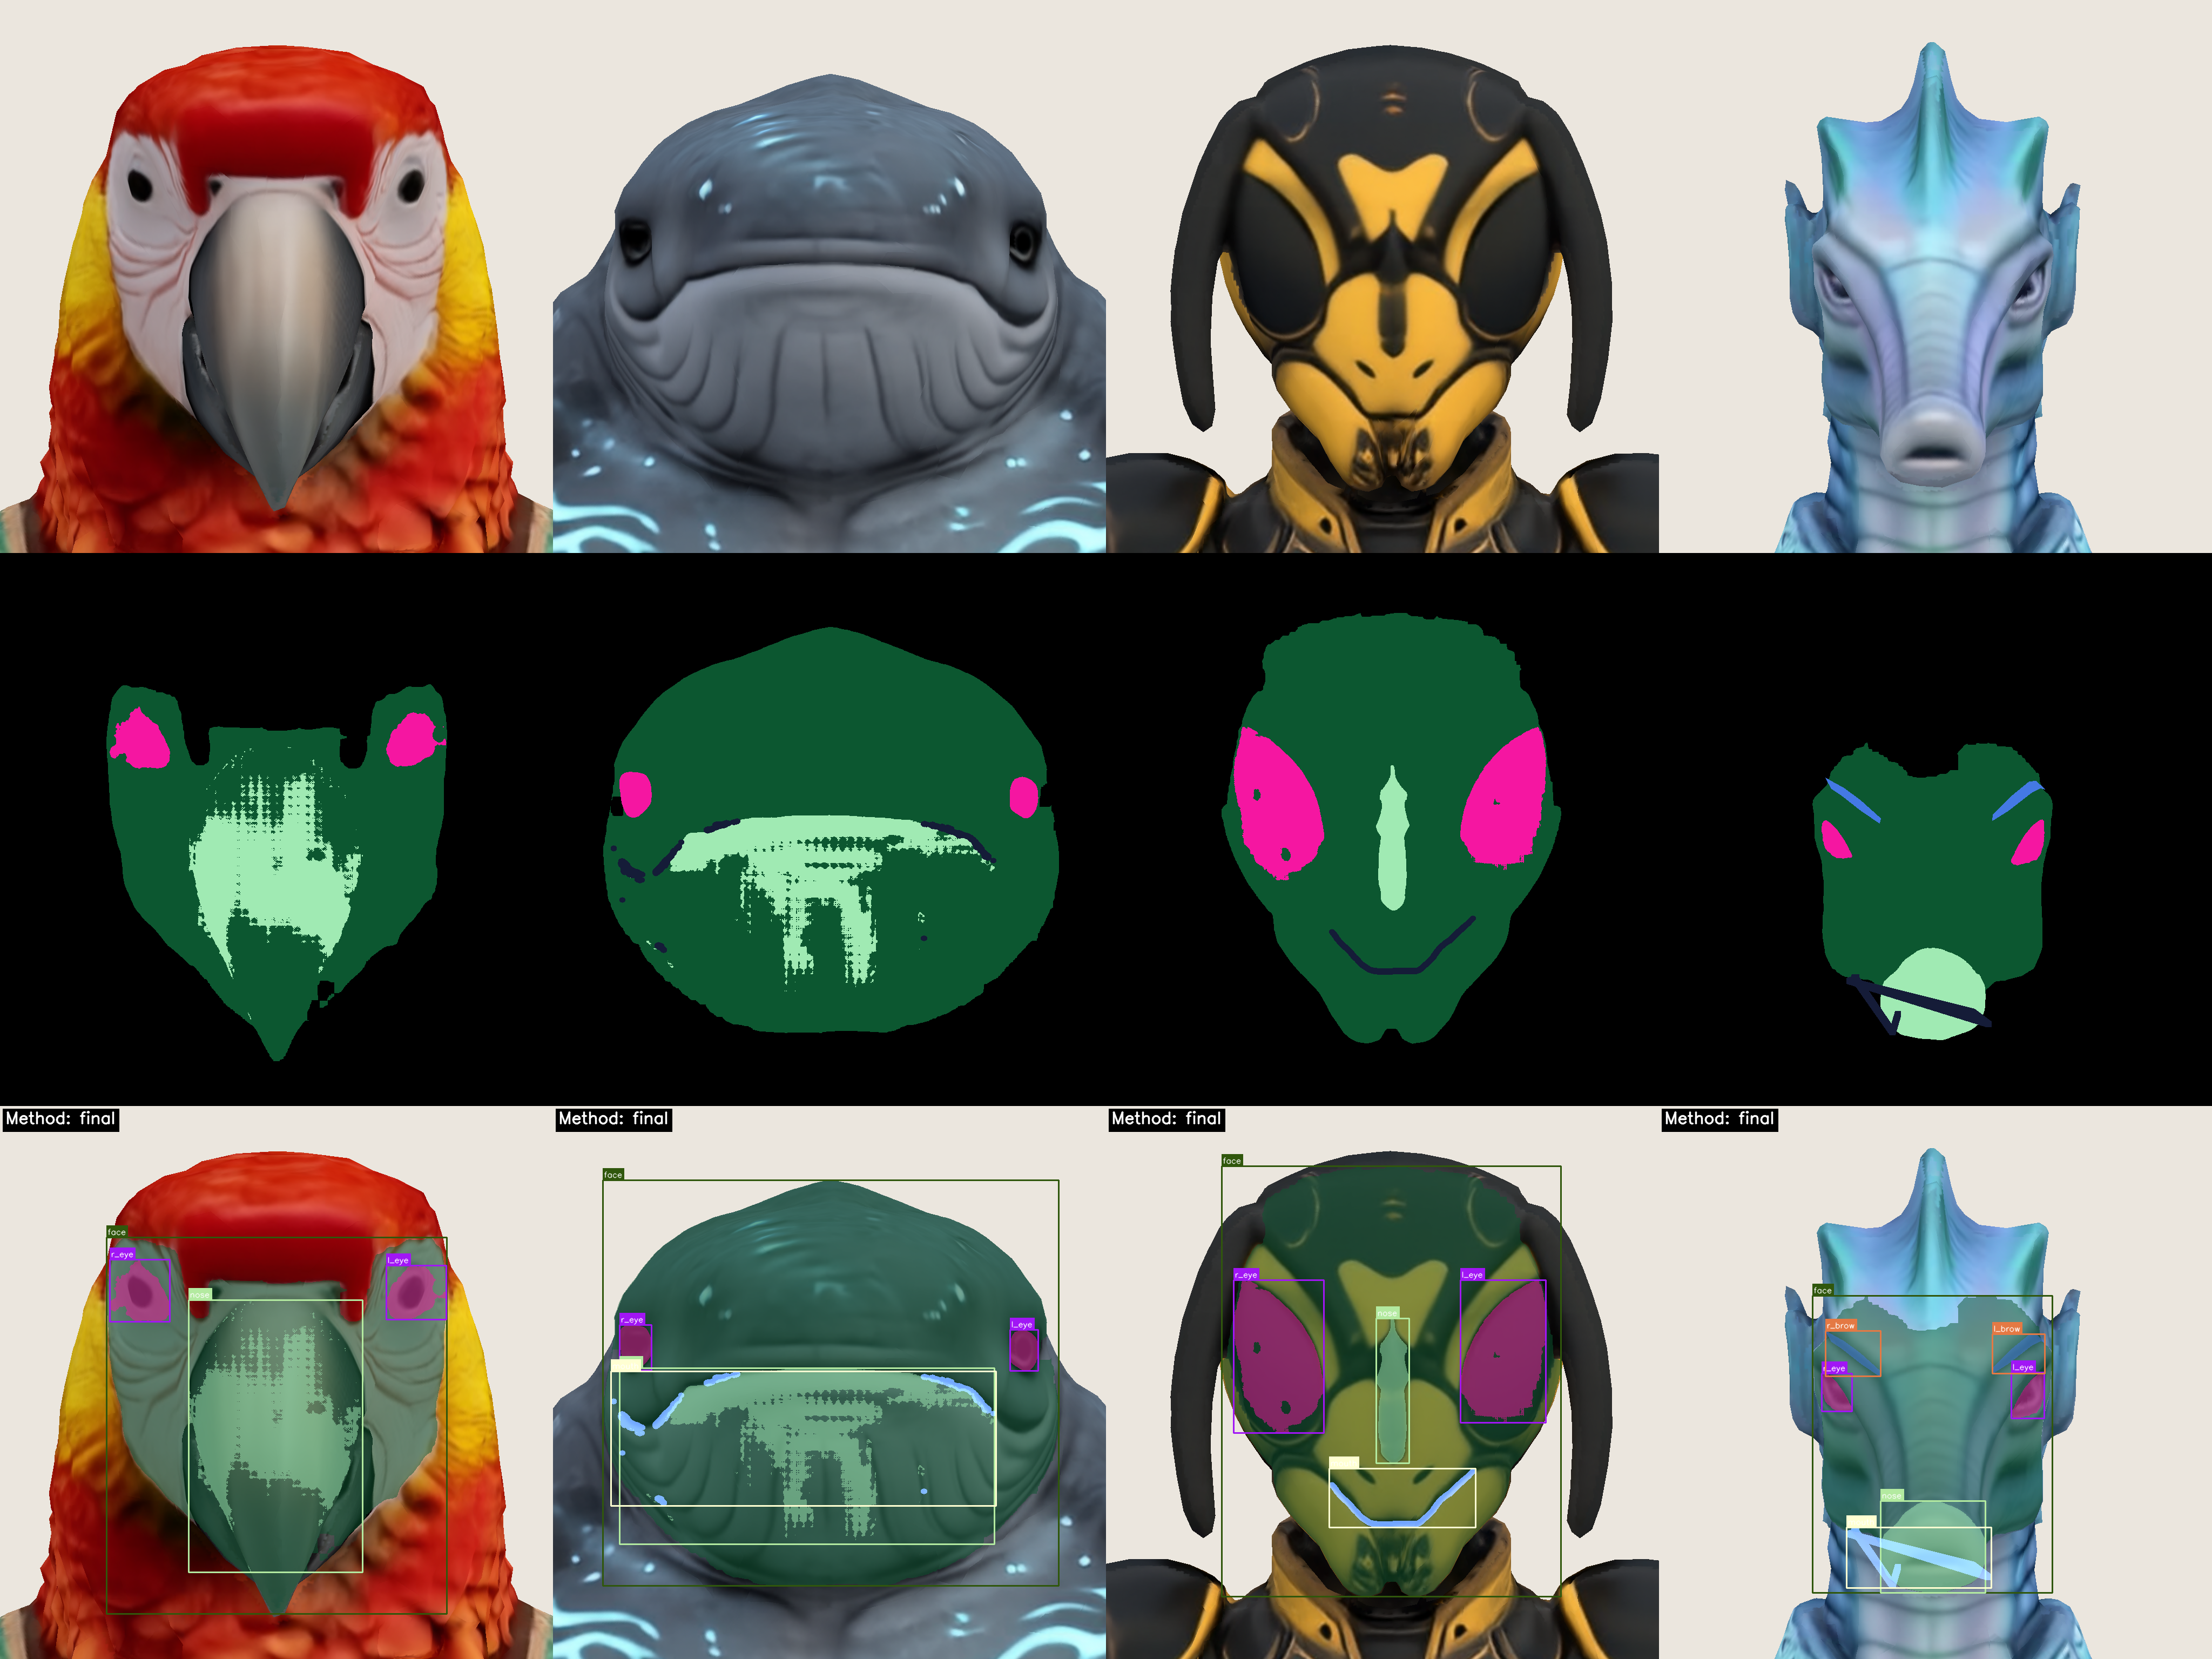
\includegraphics[width=\linewidth]{figures/failure_case.png}
  \caption{\textbf{Failure cases.} \textbf{From left to right:} (1)~a \emph{bird} with a sharp beak and an unusual surface around the beak that segmentation cannot localize as a standard face; (2)~a \emph{fish-like face} with a very wide, elongated mouth that extends almost to the face boundary, on which segmentation tends to fill in the mouth region incorrectly; (3)~an \emph{insect} with oversized compound eyes located near the face boundary and an irregular mouth layout that disrupts landmark detection; (4)~a \emph{seahorse-like animal} with a strongly elongated or flattened snout (or a heavily occluded mouth) whose facial topology falls outside our template families. \textbf{Rows (top to bottom):} input render; final segmentation mask; asset render with the mask overlaid. In all four cases, segmentation either breaks down or the underlying face/mouth anatomy cannot be reliably fit by any of our human, long-muzzle, or short-muzzle templates.}
  \Description{Four failure-case characters (bird, fish, insect, seahorse-like) arranged in 4 columns and 3 rows (input render, segmentation mask, overlay).}
  \label{fig:failures}
\end{figure}

\begin{figure*}[!p]
  \centering
  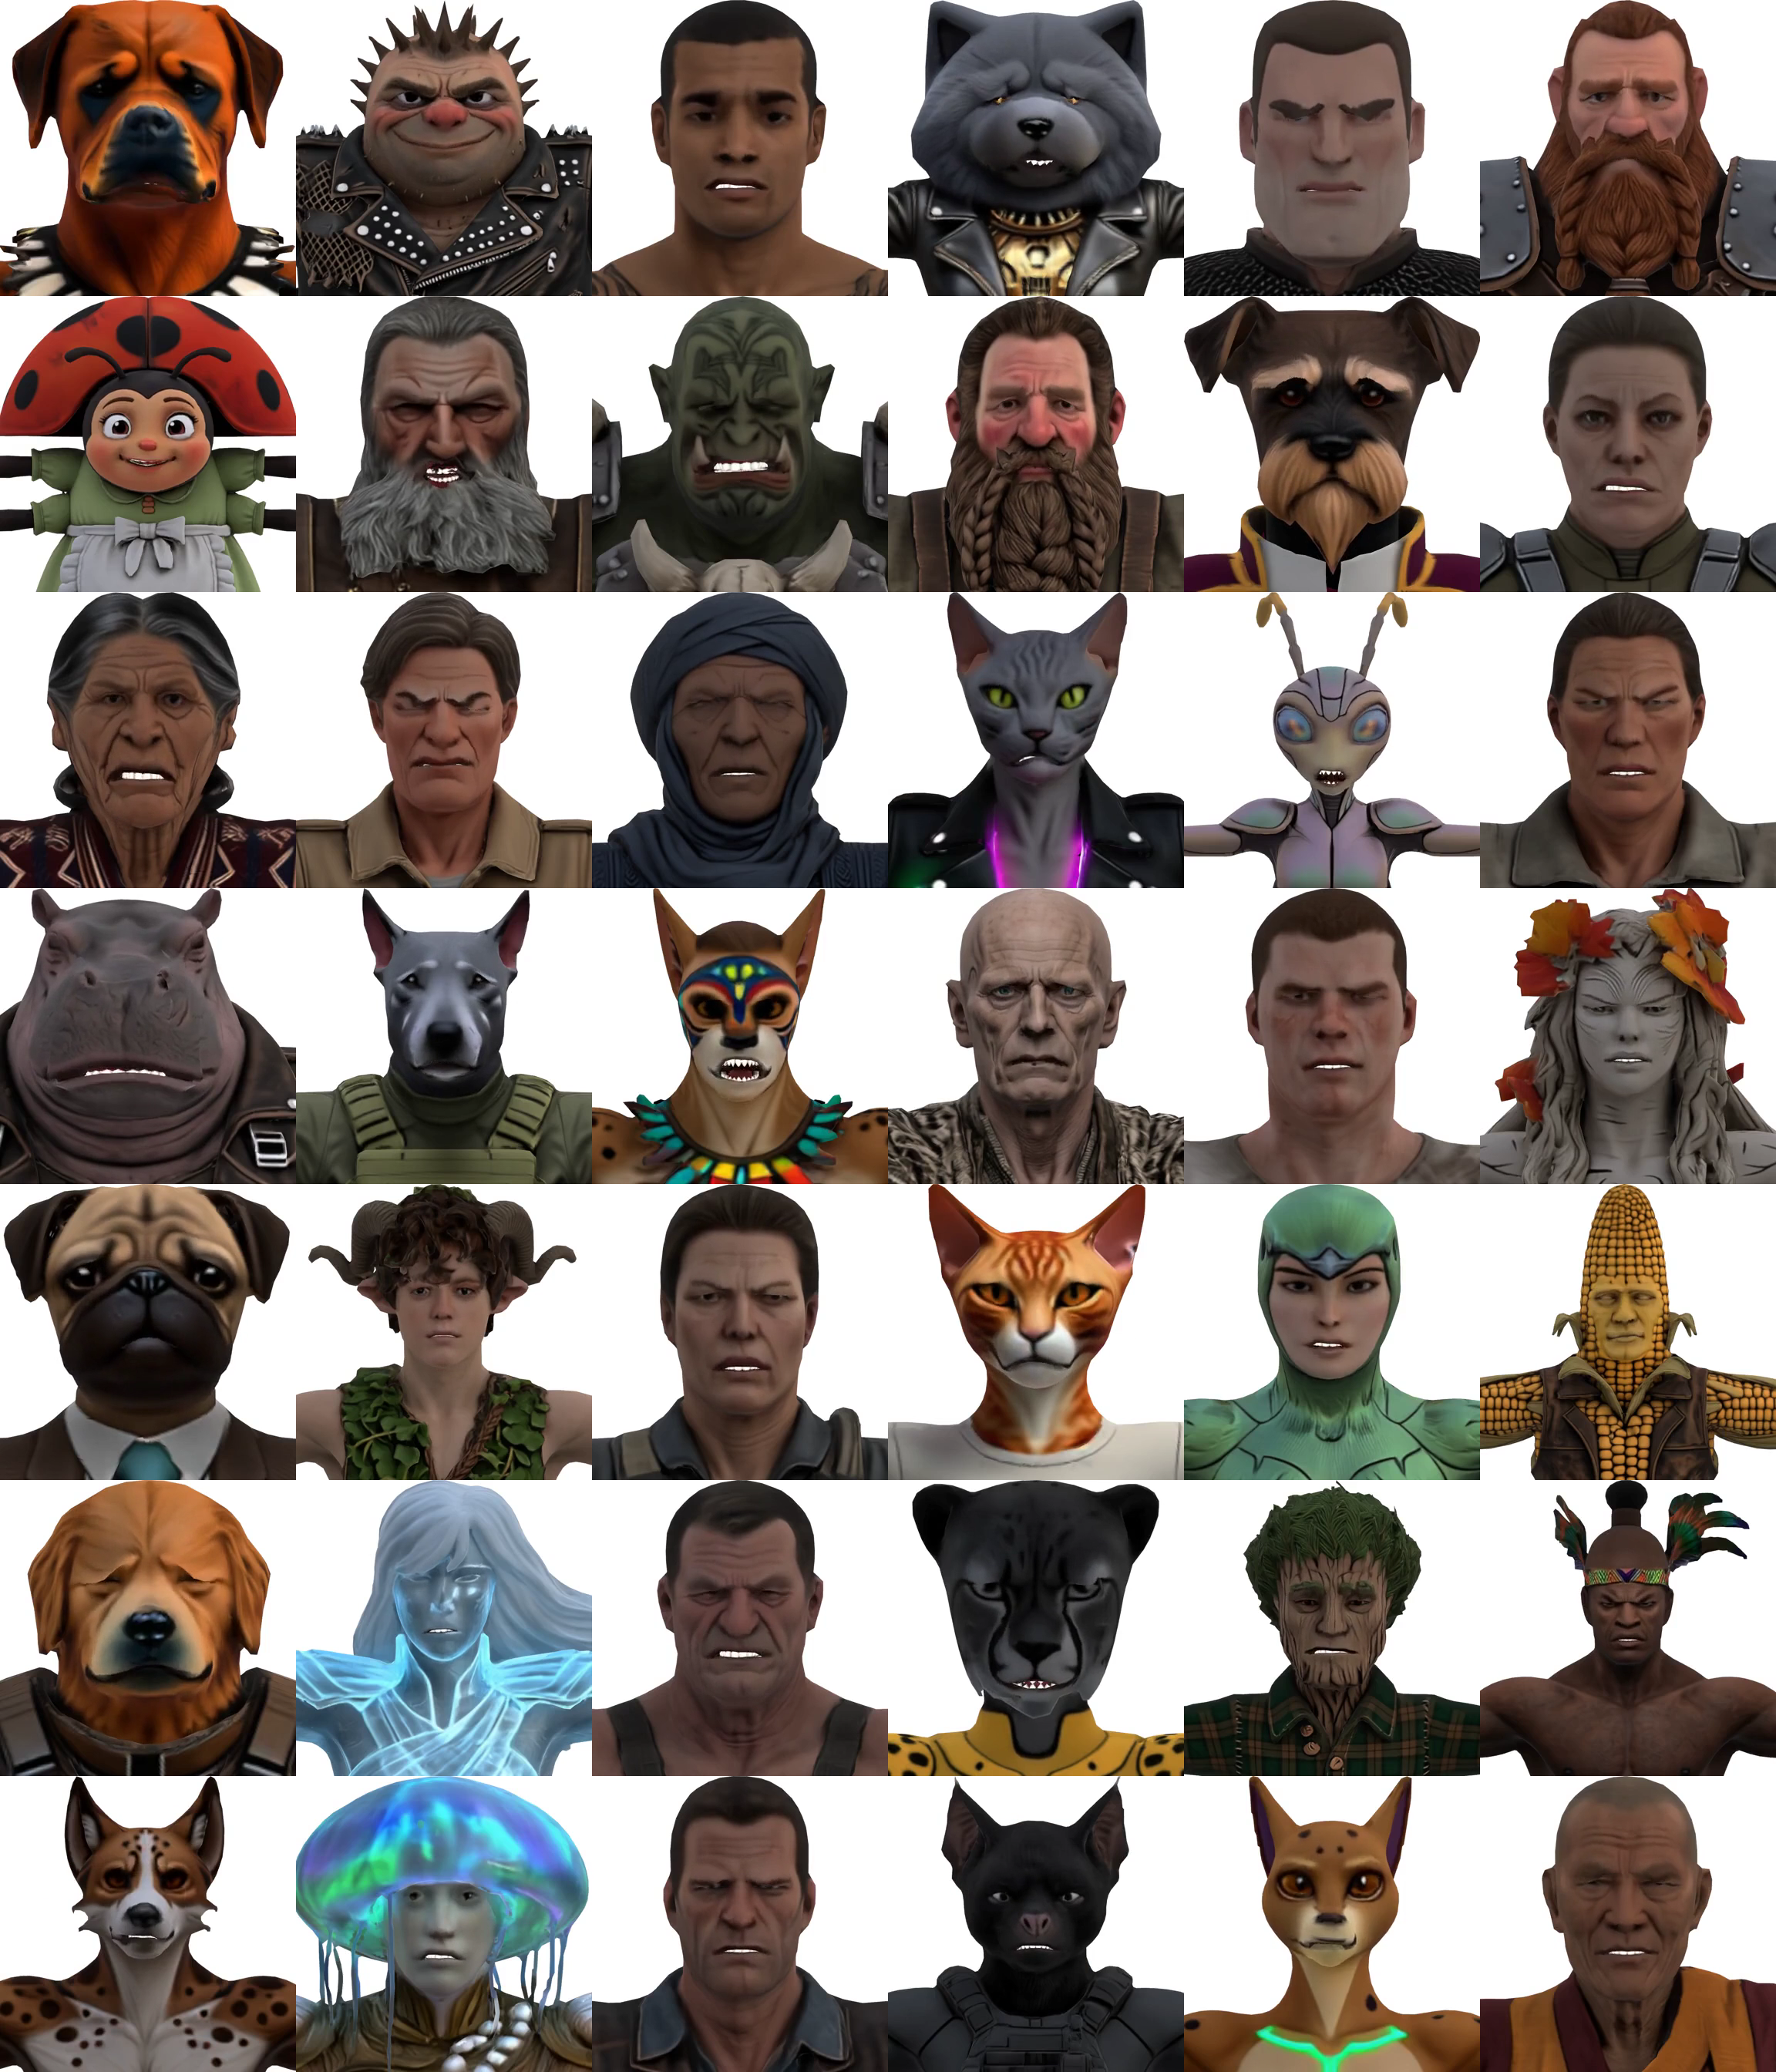
\includegraphics[width=0.95\textwidth]{figures/omnibench_dataset.png}
  \caption{\textbf{Omni-Bench dataset overview.} A sample grid of representative characters from Omni-Bench, spanning humans, humanoids, cats, dogs, and other animals. Each cell shows a rendered frame of the \emph{rigged} asset produced by OmniFaceRig, with the expression sampled at random from the FACS rig (not the static input mesh). Omni-Bench contains 1,000 rigged biped 3D characters in T-pose, each with an automatically generated FACS facial rig, inner-mouth geometry (teeth, gums, tongue), and full text-to-3D generation metadata.}
  \Description{A grid of representative Omni-Bench characters covering humans, humanoids, cats, dogs, and other animals, shown as rendered frames of their automatically rigged outputs with randomly sampled expressions.}
  \label{fig:omnibench_overview}
\end{figure*}

\begin{figure*}[!p]
  \centering
  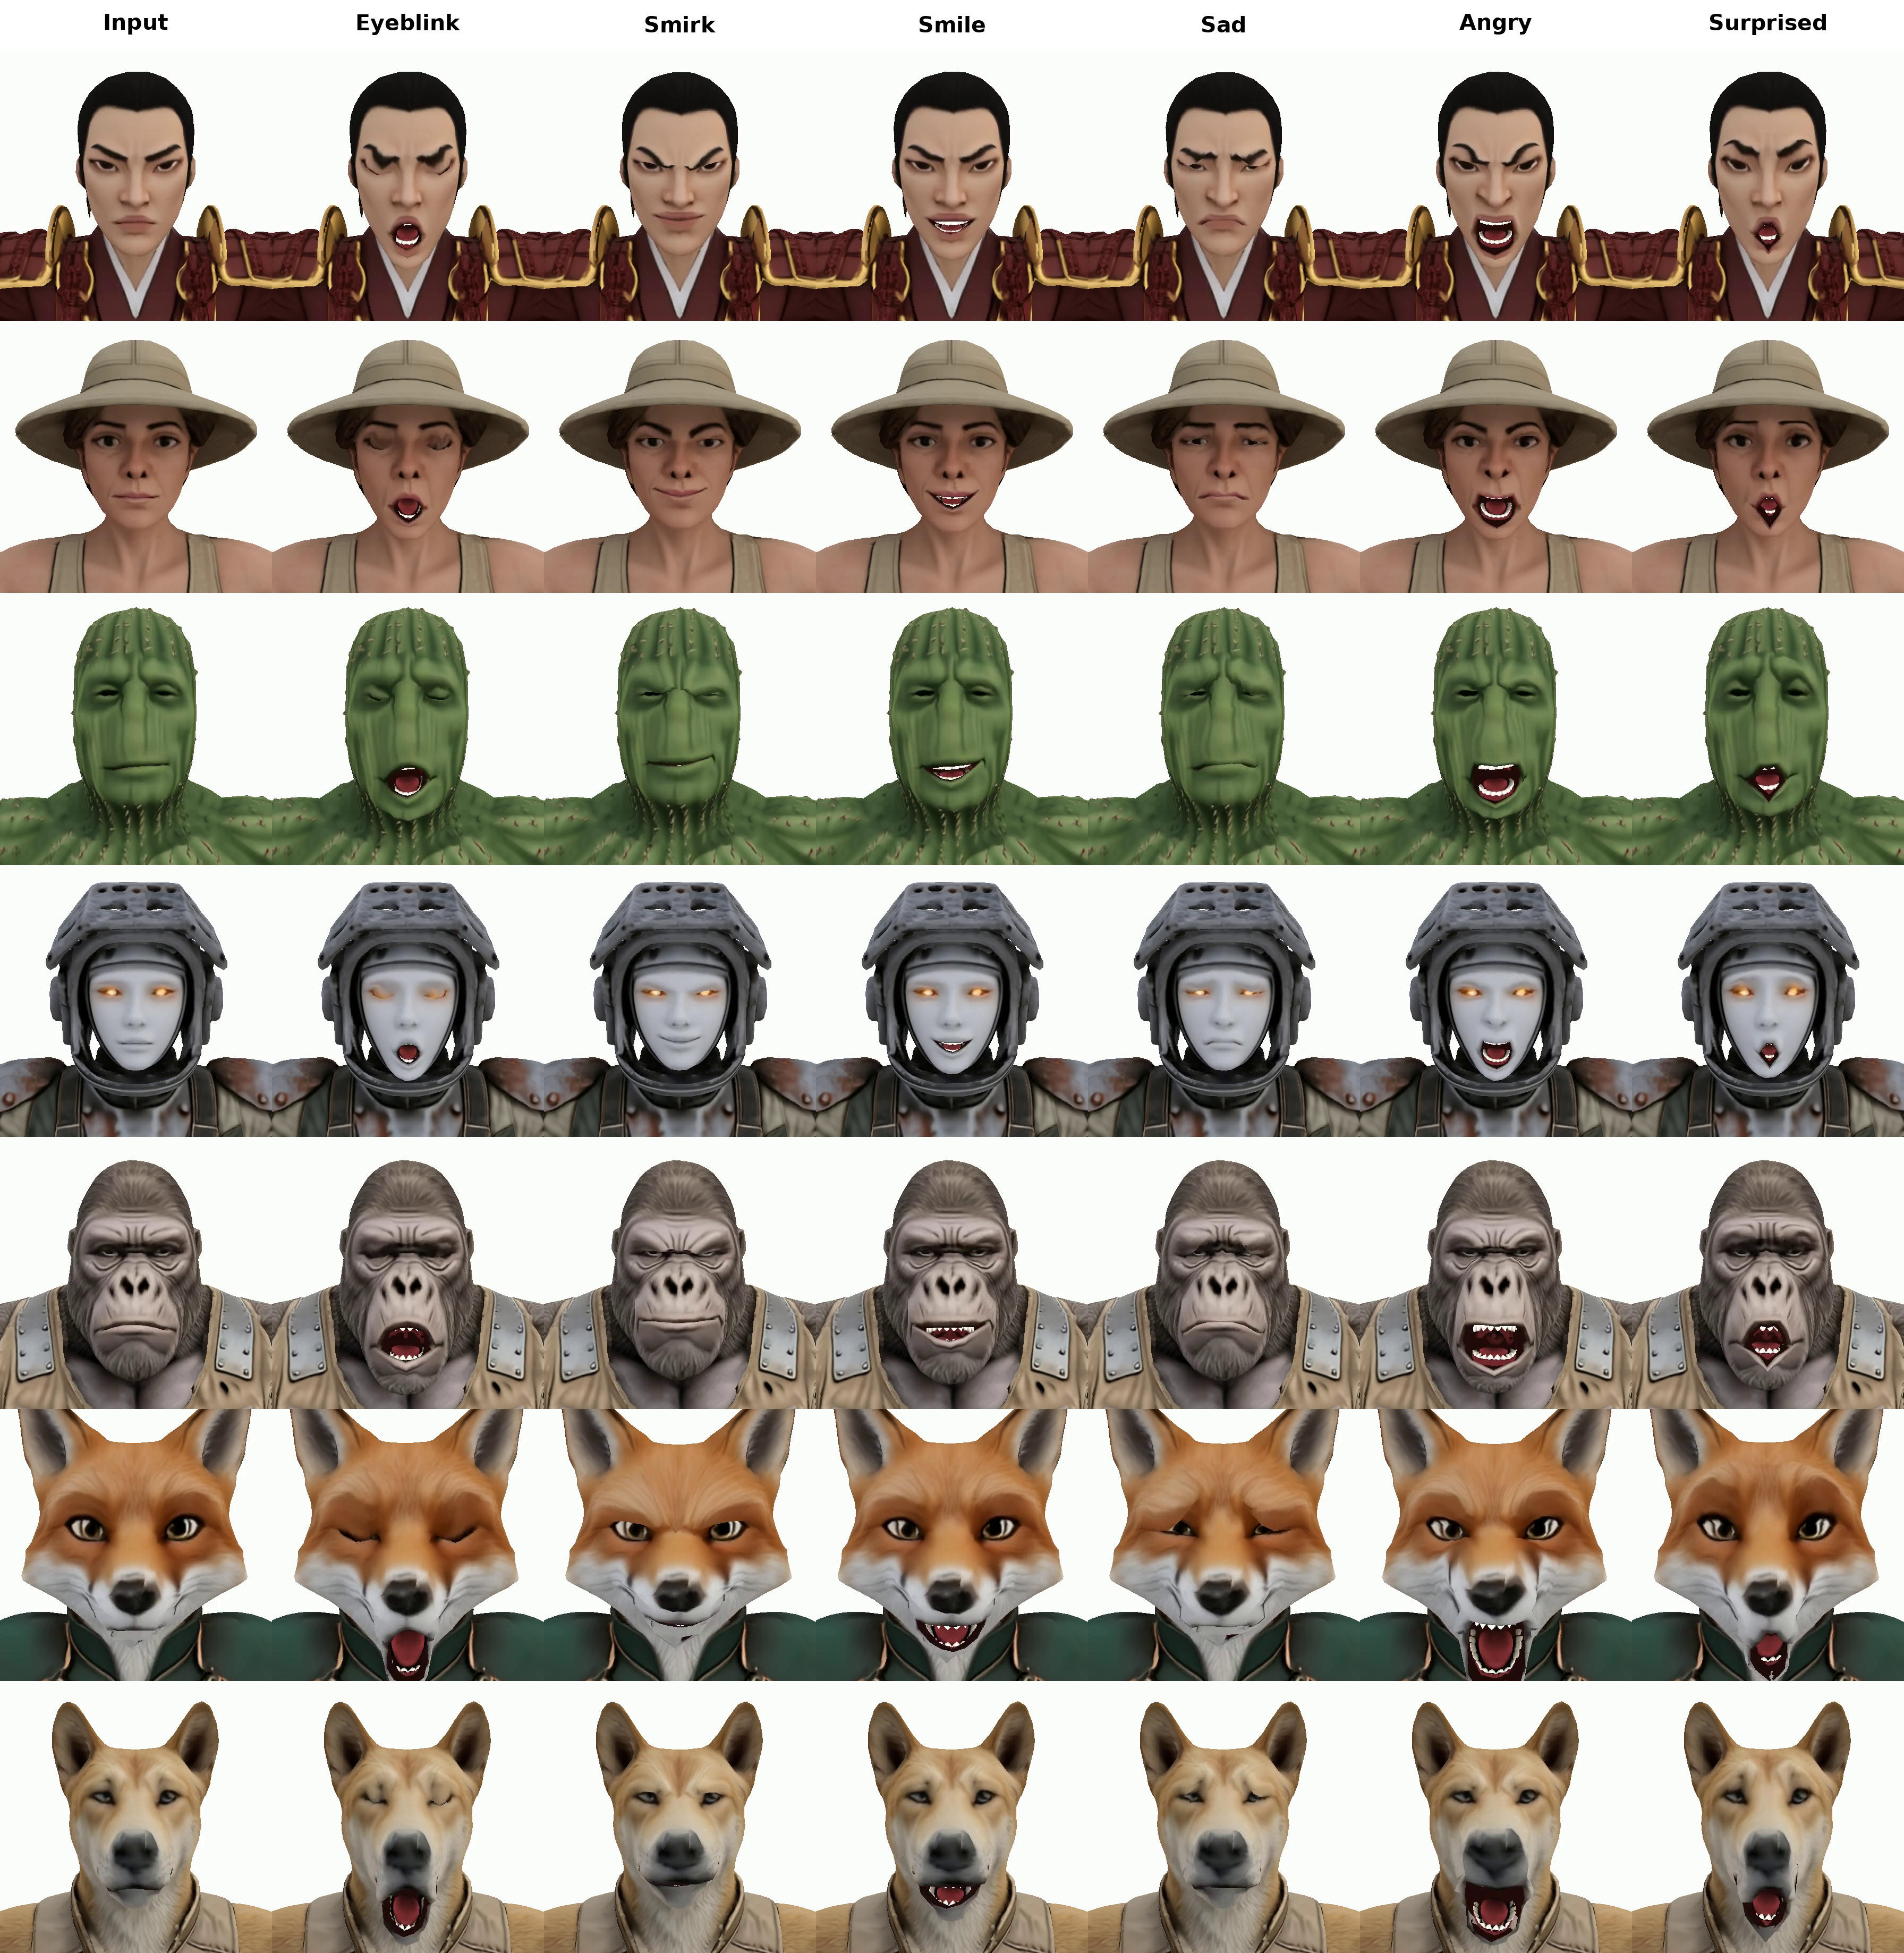
\includegraphics[width=\textwidth]{figures/main_result.png}
  \caption{\textbf{Qualitative OmniFaceRig results across diverse 3D characters from Omni-Bench.} Each row is one character. The leftmost column is the input \emph{static surface-only mesh with no pre-modeled oral cavity} (no teeth, gums, tongue, or animation-grade facial topology). The remaining six columns are generated expression frames from the OmniFaceRig output, labeled at the top (e.g., \emph{surprise}, \emph{smile}, \emph{love}); most involve open-mouth deformations that expose the \emph{procedurally generated inner-mouth geometry}. Spanning humans, humanoids, long-muzzled animals (dogs, wolves, foxes), and short-muzzled animals (cats, bears, tigers), the same fully automatic pipeline produces complete FACS rigs from a surface-only input, keeps teeth and face intersection-free via ARAP+SDF placement, and preserves character-specific identity through sparse deformation transfer---generalizing across diverse 3D character topologies \emph{without any per-asset manual authoring}.}
  \Description{Qualitative results grid showing rows of input assets and their generated expression frames across humans, humanoids, long-muzzled animals, and short-muzzled animals.}
  \label{fig:qualitative_results}
\end{figure*}

\subsection{Ablation Studies}

\textbf{Segmentation Model Ablation.} We evaluate the contribution of each model in our four-model ensemble by measuring face detection recall on Omni-Bench when using each model individually versus the full ensemble (Table~\ref{tab:seg_ablation}).

\begin{table}[t]
  \caption{Ablation: segmentation model contribution. Face detection recall (\%) on Omni-Bench. The four-model ensemble achieves nearly perfect recall by combining each model's strengths.}
  \label{tab:seg_ablation}
  \begin{tabular}{lcccc}
    \toprule
    Model Config & Human & Cat & Dog & Overall \\
    \midrule
    Face landmark only & 92\% & 12\% & 18\% & 41\% \\
    Sapiens only & 88\% & 35\% & 42\% & 55\% \\
    SAM 3 only & 78\% & 71\% & 68\% & 72\% \\
    Fine-tuned Sapiens only & 90\% & 89\% & 85\% & 88\% \\
    \textbf{4-model ensemble (Ours)} & \textbf{100\%} & \textbf{100\%} & \textbf{97\%} & \textbf{$\sim$99\%} \\
    \bottomrule
  \end{tabular}
\end{table}

Face landmark detection provides high precision on human faces (92\%) but fails almost entirely on animals (12--18\%), as it is trained exclusively on human face data. Standard Sapiens degrades on non-human faces (35--42\%) due to its human-centric training, despite being a strong foundation model. SAM 3 offers the broadest single-model coverage (72\% overall) due to its class-agnostic design, but provides coarser segmentation boundaries than landmark-based methods. Fine-tuned Sapiens substantially improves animal face detection (85--89\%) while retaining strong human performance (90\%), validating the effectiveness of our fine-tuning strategy. The four-model ensemble with adaptive per-region selection achieves nearly 100\% overall recall by combining the precision of face landmark detection on humans, fine-tuned Sapiens' robustness on animals, and SAM 3's fallback coverage for edge cases.

\textbf{Nose Landmark Ablation.} We evaluate the impact of our nose-landmark-free template design on animal face rigging quality. When nose anchor keypoints are included (as in prior template designs), the pipeline produces severely distorted nose-mouth regions on 78\% of animal assets and crashes on 10\%, driven by the two failure modes discussed in \S\ref{sec:fitting}: incorrect nose segmentation, and---even when the nose mask is plausible---unstable keypoints from uniform boundary sampling on small, irregular nose contours. Removing nose anchors and allowing the optimization to position the nose region from the surrounding border, eye, and mouth anchors eliminates these distortion artifacts and reduces the crash rate to \textbf{0\%} across all animal assets in Omni-Bench. Figure~\ref{fig:nose_rationale} provides visual evidence for both failure modes across a range of character topologies.

\textbf{Riggability Checker.} The hybrid VLM+CV approach outperforms either component alone (Table~\ref{tab:riggability}): the VLM provides strong archetype identification and accessory detection, while CV filtering catches geometric edge cases (no-face assets, degenerate meshes).


\subsection{Latency Breakdown}
\label{sec:latency}

The face pipeline executes on a single NVIDIA A100 GPU. End-to-end latency is approximately 20--30\,s per asset, including data I/O. Stage~1 (riggability assessment, face parsing, keypoint extraction, and template fitting) takes 8--10\,s, while Stage~2 (mesh fusion, inner-mouth fitting, UV/texture processing, and blendshape transfer) takes 10--15\,s. Compared to manual sculpting workflows that typically take hours to days, this represents a reduction of 2--3 orders of magnitude.


%% ============================================================
\section{Limitations and Future Work}
\label{sec:limitations}

While OmniFaceRig significantly advances automatic facial rigging, it still has limitations. The current system is designed for visible-faced characters whose facial topology falls within our human, long-muzzle, and short-muzzle template families. Specialized animals with qualitatively different mouth and face anatomy---for example birds with sharp beaks, fish-like faces with flat snouts, insects with oversized compound eyes, or animals with unusually elongated snouts (Figure~\ref{fig:failures})---may be rejected by the riggability checker or produce unreliable fits even when segmentation succeeds. More generally, our template-family design improves robustness over a single universal template, but it does not provide a fully general facial parameterization for every possible animal or stylized character; extending coverage to new topology families will require additional templates, segmentation labels, and riggability criteria. Finally, although the 20--30\,s runtime is fast relative to manual rigging, the current multi-stage pipeline is still better suited for offline or batch asset processing than real-time interactive editing. Future work will explore broader topology families, more adaptive template generation, and tighter integration of the perception and geometry stages. Additional riggability-checker failure modes (annotation borderline cases and VLM-only semantic errors) are illustrated in the supplemental material.

%% ============================================================
\section{Conclusion}
\label{sec:conclusion}

We presented OmniFaceRig, a fully automatic inner-mouth-aware face rigging pipeline for 3D characters. Given a static surface-only 3D mesh with no pre-modeled oral cavity, OmniFaceRig produces a production-ready rig with up to 155 FACS blendshapes and procedurally generated inner-mouth geometry (teeth, gums, and tongue), with no manual intervention at any stage. Our four-model detection and segmentation ensemble, combined with a nose-landmark-free template design, enables robust fitting across diverse 3D character topologies---humans, humanoids, long-muzzled animals, and short-muzzled animals---with sub-millimeter alignment error and zero pipeline crashes across all animal assets in Omni-Bench, while ARAP+SDF teeth placement keeps inner-mouth geometry intersection-free even for muzzled species. We also release Omni-Bench, to our knowledge the first open benchmark of 1,000 rigged biped characters with FACS facial blendshapes and inner-mouth geometry, to catalyze future research in automatic facial rigging.

%% ============================================================
\begin{acks}
% Acknowledgments will be added after the review process.
\end{acks}

\bibliographystyle{ACM-Reference-Format}
\bibliography{references}

\end{document}

% Supplementary material moved to supplemental.tex.

\appendix

\section{Supplementary Riggability Assessment Details}
\label{app:riggability}

This appendix expands the design of the hybrid riggability checker introduced in \S\ref{sec:riggability}. We give the per-question signal assignment, the geometric thresholds used to validate segmentation masks, the landmark-based mouth-quality gate, the three-signal fusion logic, and a brief discussion of the remaining failure modes that bound the accuracy of the gate.

\subsection{VLM+CV Signal Architecture}

The checker fuses one semantic signal and two CV-derived signals computed from a single rendered view of the input asset:

\begin{itemize}
  \item \textbf{VLM semantic signal.} A state-of-the-art Vision-Language Model answers a fixed set of high-level questions about the rendered character (face type, number of faces, eye orbits, accessories, mouth state, teeth visibility). These questions capture failure modes that are inherently semantic and hard to phrase as geometric thresholds.
  \item \textbf{Segmentation-mask signal.} The face/eye/mouth masks produced by the segmentation ensemble (\S\ref{sec:segmentation}) are evaluated against geometric plausibility criteria: presence of each region, inclusion inside the face boundary, plausible eye-to-head ratio, and acceptable lip-seal curvature.
  \item \textbf{Landmark-quality signal.} For human-like faces, the regularity of mouth landmarks is summarized by a lip-evenness statistic and used as a quality gate before mouth evidence enters the fusion step.
\end{itemize}

The three signals are not treated as redundant: each question in the underlying checker template is assigned to the signal that is empirically most reliable for it, as summarized in Table~\ref{tab:rigg_questions}.

\begin{table}[h]
  \caption{Per-question signal assignment in the riggability checker. ``VLM'' uses the semantic signal alone; ``Seg mask'' replaces a VLM yes/no question with a direct geometric measurement; ``Majority'' fuses VLM, segmentation, and landmark evidence with a three-way vote.}
  \label{tab:rigg_questions}
  \small
  \begin{tabular}{cll}
    \toprule
    \textbf{Q\#} & \textbf{Aspect checked} & \textbf{Signal source} \\
    \midrule
    Q1 & Face type (human / animal / other)        & VLM \\
    Q2 & Number of visible faces                  & VLM \\
    Q3 & Number of visible eye orbits             & VLM \\
    Q4 & Mouth present and localizable            & Majority \\
    Q5 & Eye-region occlusion or obstruction      & Seg mask \\
    Q6 & Eyewear covering eyes                    & VLM \\
    Q7 & Mouth state                              & VLM \\
    Q8 & Teeth visibility                         & VLM \\
    Q9 & Eye-to-head size ratio                   & Seg mask \\
    Q10 & Lip-seal curvature                      & Seg mask \\
    \bottomrule
  \end{tabular}
\end{table}

\subsection{Geometric Criteria from Segmentation Masks}

The segmentation-based checks (Q5, Q9, Q10, plus mask inclusion tests) are summarized in Table~\ref{tab:rigg_seg}. The thresholds are calibrated once on a development split and held fixed across all evaluations; they are deliberately conservative so that the checker rejects mostly inputs that would otherwise crash or distort the downstream registration stage.

\begin{table}[h]
  \caption{Geometric criteria evaluated on the face, eye, and mouth segmentation masks. Each criterion produces a binary pass/fail signal that participates in the hybrid decision.}
  \label{tab:rigg_seg}
  \small
  \setlength{\tabcolsep}{4pt}
  \begin{tabular}{@{}l p{0.58\linewidth}@{}}
    \toprule
    \textbf{Criterion} & \textbf{Pass condition} \\
    \midrule
    Mask presence            & face/eye/mouth masks non-empty \\
    Eye inclusion            & eye mask inside face boundary \\
    Mouth inclusion          & mouth mask inside face boundary \\
    Eye-region occlusion (Q5) & occluder overlap with eye region below threshold \\
    Eye-to-head ratio (Q9)   & eye/head area ratio in range \\
    Mouth curvature (Q10)    & lip-seal curvature in range \\
    \bottomrule
  \end{tabular}
\end{table}

\subsection{Landmark-Assisted Mouth Validation}

For human-like inputs, we use mouth landmarks as a quality gate before they are fused with the VLM and segmentation signals. Let $\mathrm{CV}_{\mathrm{lip}}$ denote the coefficient of variation of the spacing between consecutive lip-contour landmarks. We mark the mouth landmarks as unreliable when $\mathrm{CV}_{\mathrm{lip}}$ exceeds a calibrated threshold; the underlying intuition is that on assets with a poorly modeled or absent mouth, the landmark detector still emits points, but those points become irregularly spaced. Failing the gate sets the landmark mouth evidence to ``unavailable'' for the subsequent fusion step.

For non-human assets, where human-trained mouth-landmark detectors are not reliable, the landmark signal is ignored and the mouth decision is determined by the VLM and the segmentation mask alone.

\subsection{Mouth-Signal Fusion Logic}

The final eligibility decision is the conjunction of all per-question results in Table~\ref{tab:rigg_questions}. Q1--Q3 and Q6--Q8 are decided directly by the VLM; Q5, Q9, Q10 are decided by the segmentation-mask checks in Table~\ref{tab:rigg_seg}; and Q4 (mouth presence) uses explicit fusion because mouth localization is one of the most common downstream failure sources.

Concretely, for a human-like asset, the mouth decision is:
\begin{enumerate}
  \item If $\mathrm{CV}_{\mathrm{lip}}$ exceeds the landmark-quality threshold, treat the landmark evidence as unreliable and rely on the VLM and segmentation signals.
  \item Otherwise, take a majority vote over (i) the VLM mouth prediction, (ii) the segmentation-based mouth-detected flag, and (iii) the landmark-based mouth-detected flag.
\end{enumerate}
For non-human assets, the same step degenerates to a conjunction of the VLM and segmentation-mask signals. The majority-vote design recovers the cases that a strict ``VLM \emph{and} segmentation'' rule would miss when exactly one of the two signals is wrong but the other two agree.

\subsection{Discussion of Remaining Failure Modes}

Empirically, the hybrid VLM+CV checker on the mixed riggability validation set exhibits two dominant failure categories. The first is \emph{annotation borderline cases}, where the ground-truth label itself is ambiguous (e.g., partially occluded faces or stylized characters that are arguably riggable). The second is \emph{VLM-only semantic errors}: misclassification of eyewear, mouth state, or teeth visibility---attributes that segmentation masks and landmarks only partially corroborate. These are the natural targets for future improvement of the checker, since the geometric and landmark signals have already absorbed most of the failures they are capable of catching.

\begin{figure}[!htb]
  \centering
  \fbox{\parbox{0.95\linewidth}{\centering\vspace{2em}
  \textcolor{red}{\textbf{[TODO: RIGGABILITY FAILURE CASES]}}\\[0.4em]
  \small Placeholder for representative false-positive and false-negative examples, annotated by dominant failure source.
  \vspace{2em}}}
  \caption{\textcolor{red}{TODO: replace this placeholder with representative riggability-checker failure cases.} The final figure should show borderline cases and VLM-only semantic errors, such as ambiguous facial occlusion, eyewear/mask confusion, or mouth/teeth-state misclassification.}
  \Description{Placeholder for representative riggability-checker failure cases.}
  \label{fig:rigg_failures}
\end{figure}


\section{Supplementary Stage-2 Rig Construction Details}
\label{app:stage2}

This appendix expands the four steps of Stage~2 introduced in \S\ref{sec:blendshape}---face-region fusion, inner-mouth construction, texture/UV transfer, and blendshape transfer with post-processing. The shared difficulty across all four steps is that the input asset is surface-only: there is no pre-modeled oral cavity, no animation-grade facial topology, and no separation between expressive and structural regions.

\subsection{Face-Region Fusion}

The fitted face mesh produced by Stage~1 defines the region of the input asset that will be replaced. A high-quality animated topology---designed with radial edge loops around the eyes and mouth---is first aligned to the fitted template through their shared UV correspondence, then reprojected onto the input surface so that it inherits the asset's own facial geometry. The original face region of the input is removed via a Boolean operation against a convex hull of the fitted region, the new animated topology is inserted in its place, and the boundary between the new face and the rest of the asset is stitched by closest-point welding followed by small-edge collapse to clean up degenerate polygons. This operation is intentionally local: it preserves the asset's identity, hairstyle, and non-face geometry while introducing the radial edge flow that downstream expression deformation relies on.

\subsection{Inner-Mouth Construction}

Because the input contains no oral cavity, the inner-mouth geometry (teeth, gums, and tongue) must be synthesized rather than registered. We maintain a small library of inner-mouth template archetypes, summarized in Table~\ref{tab:teeth_archetype}; the appropriate archetype is selected by the VLM during Stage~1 from the rendered view of the character.

\begin{table}[h]
  \caption{Inner-mouth template archetypes and their typical targets. The VLM in Stage~1 selects one archetype per asset, which determines the teeth/gum/tongue template that is warped into the fitted mouth cavity.}
  \label{tab:teeth_archetype}
  \small
  \begin{tabular}{ll}
    \toprule
    \textbf{Archetype} & \textbf{Typical target characters} \\
    \midrule
    Human    & realistic humans and humanoid characters \\
    Canine   & long-muzzled animals (e.g., dogs, wolves, foxes) \\
    Monster  & stylized fantasy creatures with non-standard teeth \\
    Flat     & characters with minimal or absent oral structure \\
    \bottomrule
  \end{tabular}
\end{table}

The selected archetype is first warped into the fitted mouth cavity via smooth geometric deformation, then aligned by a rigid transform with anisotropic scale. To prevent the synthesized teeth from protruding through the outer face surface---a frequent failure case for long-muzzled animals when a human-shaped template is reused na\"ively---we apply two consecutive collision-aware refinements: an as-rigid-as-possible step that preserves the internal structure of the teeth and gums, followed by a signed-distance-field step that pushes any facial surface points that fall inside the inner-mouth volume outward along the SDF gradient. Gum and tongue geometry are fitted alongside the teeth so that they share a consistent oral-cavity envelope.

\subsection{Texture and UV Transfer}

After the new face and inner-mouth surfaces are inserted, the global UV layout is rebuilt. The face region is allocated a larger fraction of the texture domain than non-face regions so that high-frequency facial detail is preserved at any rendering resolution, and the inner-mouth surfaces are placed on a separate texture channel to keep their material parameters independent. The asset's original appearance is then transferred onto the rebuilt UV layout by sampling the original texture through the geometric correspondence between the original and merged surfaces; this preserves the character's identity and material details while letting the newly synthesized geometry inherit a coherent appearance.

\subsection{Blendshape Transfer and Post-Processing}

FACS expression shapes are produced by transferring local deformation gradients from a canonical rigged template to the merged character mesh using sparse deformation transfer. Adapting the deformation gradients to the target character's own proportions is what keeps the transferred expressions character-specific rather than collapsing the rig toward an ``average human face,'' and is what allows the same set of FACS shapes to be applied to humans, humanoids, long-muzzled animals, and short-muzzled animals without per-character authoring.

The transferred deformations are then blended outward from the facial template region into the adjacent head surface so that expression motion fades smoothly into the rest of the asset. Sparse deformation transfer alone cannot enforce certain physical and geometric constraints---eyelids must close without self-intersection, eye-gaze shapes require a known rotation center, jaw motion must move the lower teeth, and extreme mouth poses can re-introduce teeth-face intersections. A small set of expression-specific post-processing rules, summarized in Table~\ref{tab:postprocessing}, handles these cases.

\begin{table}[h]
  \caption{Expression-specific post-processing rules applied after sparse deformation transfer. Each rule addresses a constraint that pure deformation transfer cannot enforce on its own.}
  \label{tab:postprocessing}
  \small
  \setlength{\tabcolsep}{4pt}
  \begin{tabular}{@{}l p{0.58\linewidth}@{}}
    \toprule
    \textbf{Shape category} & \textbf{Refinement applied} \\
    \midrule
    Closed-eye shapes        & upper-eyelid vertices snapped to lower lid and locally relaxed for contact-aware closure \\
    Eye-gaze shapes          & eye-region vertices rotate around virtual eyeball centers from Procrustes fit \\
    Jaw-related shapes       & lower-teeth subset moves coherently with the jaw, tracking open/close motion \\
    Collision-aware refinement & SDF-based teeth-face penetration check re-applied per expression shape \\
    \bottomrule
  \end{tabular}
\end{table}

\subsection{Design Tradeoffs and Outlook}

The four steps of Stage~2 are coupled but decomposable: face-region fusion fixes the surface topology, inner-mouth construction synthesizes the missing oral cavity, UV/texture transfer preserves the character's original appearance, and blendshape transfer turns the static rig into an animatable one. A common thread is that each step substitutes a procedural geometric operation for what is traditionally a manual authoring step, which is also what makes the full pipeline fully automatic.

The two design choices that most directly enable cross-topology generalization are the use of multiple inner-mouth archetypes (Table~\ref{tab:teeth_archetype}) and the SDF-based collision refinement at both the rest pose and the per-expression level. Without the archetype split, a single human-shaped teeth template either intersects long muzzles or sits too far back in flat-faced animals; without the SDF refinement, expression shapes such as a wide jaw open or a strong smile can re-introduce intersections that the rest-pose placement avoids. Together with the topology-specific face templates of Stage~1, these choices let the same Stage~2 procedure produce rigs for humans, humanoids, long-muzzled animals, and short-muzzled animals without any per-category authoring.

Together, the four steps of Stage~2 turn a static, surface-only 3D character mesh---without any pre-modeled oral cavity, without any animation-grade facial topology, and without any per-character authored expressions---into a full inner-mouth-aware FACS facial rig.

\end{document}
